% =====================================================================
% Seccion: Preparacion del dataset (Hito 2)
% Fragmento SIN preambulo: se incluye con % =====================================================================
% Seccion: Preparacion del dataset (Hito 2)
% Fragmento SIN preambulo: se incluye con % =====================================================================
% Seccion: Preparacion del dataset (Hito 2)
% Fragmento SIN preambulo: se incluye con % =====================================================================
% Seccion: Preparacion del dataset (Hito 2)
% Fragmento SIN preambulo: se incluye con \input{secciones/preparacion_dataset}
% Paquetes requeridos: graphicx, booktabs, xcolor, tikz (+ calc no), pgfplots, caption
% Figuras: guia_visual_5rois.png vive en docs/guias/ (ver \graphicspath en el archivo principal)
% Las cifras salen de data/processed/etiquetado/etiquetas_revisadas.csv,
% data/processed/dataset_35k/manifest_35k.csv y de los scripts de scripts/.
% Todo lo que no se pudo verificar se marca con \pendiente{...} (se ve en rojo).
% =====================================================================
\providecommand{\pendiente}[1]{\textcolor{red}{\textbf{[PENDIENTE: #1]}}}
\providecommand{\arch}[1]{\texttt{\detokenize{#1}}}

\section{Preparación del dataset}
\label{sec:dataset}

Esta sección describe, en orden, cómo se pasó del conjunto público original a los 35\,007 recortes (ROI) con los que se entrenaron y compararon los cuatro modelos. La Figura~\ref{fig:flujo} resume el flujo y el número de elementos que pasan por cada etapa. Todas las cifras proceden de los archivos versionados del repositorio; lo que no pudo verificarse se señala como pendiente.

\begin{figure}[t]
\centering
\begin{tikzpicture}[
  box/.style={draw, rounded corners=2pt, align=left, text width=0.60\linewidth, inner sep=3pt, font=\footnotesize},
  num/.style={align=left, text width=0.30\linewidth, font=\footnotesize\bfseries},
  arrow/.style={-{Stealth[length=2mm]}, thick},
  node distance=4.2mm]
  \node[box] (a) {1. Conjunto público (Mendeley), archivos \texttt{.IMA}};
  \node[num, right=3mm of a] {575 carpetas, $\approx$48\,000 archivos};
  \node[box, below=of a] (b) {2. Descarte de series inútiles y conservación de T2 sagital};
  \node[num, right=3mm of b] {solo T2 sagital};
  \node[box, below=of b] (c) {3. Conversión DICOM$\to$PNG y limpieza manual de cortes};
  \node[num, right=3mm of c] {1\,086 cortes, 414 pacientes};
  \node[box, below=of c] (d) {4. Recorte L1--S1 y detección de discos (ROI 128$\times$128)};
  \node[num, right=3mm of d] {5\,385 ROI};
  \node[box, below=of d] (e) {5. Preetiquetado, revisión humana (A/B) y exclusiones};
  \node[num, right=3mm of e] {5\,123 ROI, 399 pacientes};
  \node[box, below=of e] (f) {6. División por paciente 70/15/15};
  \node[num, right=3mm of f] {279 / 60 / 60 pacientes};
  \node[box, below=of f] (g) {7. Aumento dentro de cada partición (balance por conteo)};
  \node[num, right=3mm of g] {35\,007 imágenes};
  \foreach \i/\j in {a/b,b/c,c/d,d/e,e/f,f/g} \draw[arrow] (\i) -- (\j);
\end{tikzpicture}
\caption{Flujo de preparación del dataset y número de elementos en cada etapa.}
\label{fig:flujo}
\end{figure}

\subsection{Origen de los datos}
Se usó el \emph{Lumbar Spine MRI Dataset} (Mendeley Data) \cite{sudirman2019}, el mismo conjunto público empleado en trabajos previos sobre clasificación de hernia discal \cite{sari2024}. Los estudios se adquirieron con un único equipo, un Siemens MAGNETOM Essenza de 1,5~T, y se distribuyen como archivos DICOM con extensión \arch{.IMA}, en una carpeta por paciente. Los cortes tienen un tamaño de píxel de 0,729~mm, un grosor de 4~mm y una separación entre centros de 4,8~mm. El campo \texttt{PatientID} está vacío en todo el corpus y el repositorio solo conserva identificadores de estudio y de serie (los campos de nombre, nacimiento y fecha están vacíos en \arch{meta_dicom_por_slice.csv}). El conjunto descargado contenía 575 carpetas de pacientes. Se eliminaron las que, en lugar de resonancia lumbar, contenían estudios del segmento cervical o de rodillas, y las lumbares con aberraciones o manchas que habrían introducido ruido en los modelos. Tras esa depuración quedaron 414 pacientes con cortes útiles y, tras las exclusiones de calidad de los ROI (Sección~\ref{sec:roi}), los \textbf{399 pacientes} del dataset final. Cada una de las 414 carpetas restantes corresponde a un \texttt{StudyInstanceUID} distinto y no se repite ningún \texttt{StudyTime}; no hay evidencia de pacientes duplicados, aunque con el identificador vacío no puede descartarse del todo.
% VERIFICAR: el sitio de Mendeley describe 515 pacientes; el equipo reporta 575 carpetas descargadas.

\subsection{Depuración de la fuente}
La descarga inicial contenía cerca de 48\,000 registros en formato \arch{.IMA}. Cada paciente trae varias series; solo una parte sirve para este problema. La Tabla~\ref{tab:descartes} lista lo que se descartó y por qué.

\begin{table}[t]
\centering\small
\caption{Series descartadas de cada estudio y motivo.}
\label{tab:descartes}
\begin{tabular}{p{0.30\linewidth}p{0.60\linewidth}}
\toprule
Serie & Motivo del descarte \\
\midrule
\arch{LOCALIZER_0001} & Localizadores de muy baja resolución usados por el técnico para calibrar la mesa y posicionar al paciente; no aportan información anatómica ni de textura. \\
\arch{POSDISP_[4]_T2_TSE_TRA_...} & Vistas sagitales con líneas blancas superpuestas (\emph{overlays}) que marcan los planos transversales; ese artefacto distorsiona descriptores de textura (GLCM/LBP) y confunde a las redes. \\
\arch{T1_TSE_SAG_...}, \arch{T1_TSE_TRA_...} & En T1 la grasa es brillante y el líquido oscuro, de modo que no permite evaluar la hidratación del disco (base de la escala de Pfirrmann); además, mezclar T1 y T2 altera los rangos de brillo. \\
\arch{T2_TSE_TRA_...} (axial) & Cortes axiales fragmentados en lotes de 3 a 5 por nivel; exigirían un emparejamiento espacial adicional por disco, mientras que el plano sagital cubre L1--S1 en una sola imagen. Se deja para una fase futura. \\
\bottomrule
\end{tabular}
\end{table}

El proceso se hizo en cuatro pasos, cada uno con su script (carpeta \arch{scripts/preprocesamiento/}):
\begin{enumerate}
  \item \arch{ingestion.py} recorre las carpetas de pacientes y copia solo las imágenes T2 sagitales, identificadas por el nombre de la serie.
  \item \arch{limpiar_slices.py} conserva el 40\,\% central del volumen sagital (se descarta el 30\,\% inicial y el 30\,\% final), donde el canal medular y la región L1--S1 son visibles.
  \item \arch{convertidor_dcm_a_png.py} convierte a PNG de 8 bits con una sola escala por serie: percentiles 1 y 99,5 calculados sobre los píxeles de tejido. Se decidió no aplicar CLAHE ni otro realce, para no alterar la señal relativa del T2 que sustenta el criterio diagnóstico.
  \item Depuración manual de los PNG: algunos pacientes tenían estudios del segmento cervical o de rodillas, y otros cortes T2 sagitales quedaban oscuros o con aberraciones; se eliminaron.
\end{enumerate}
Tras esta depuración quedaron \textbf{1\,086 cortes sagitales de 414 pacientes} (2,6 cortes por paciente en promedio; entre 1 y 6).

\subsection{Recorte de la región lumbar y de los ROI por disco}
\label{sec:roi}
\paragraph{Recorte L1--S1.} Con \arch{aplicar_recortes.py} se recortó cada corte en altura para abarcar principalmente L1--S1, replicando por \emph{template matching} unos recortes manuales previos (mediana de la puntuación de coincidencia 0,9996; solo el corte 0547\_008 quedó por debajo de 0,99). El recorte se extendió 60~px hacia arriba y hacia abajo hasta el borde de la imagen; con ello el relleno necesario en L1-L2 bajó de 779 de 1\,080 recortes (72\,\%) a cero.

\paragraph{Detector de discos.} Para localizar los discos se entrenó un detector con un conjunto propio en Roboflow (proyecto \emph{Intervertebral Disks}, versión~1): 100 cortes (70 de entrenamiento, 20 de validación y 10 de prueba), con orientación automática (\emph{auto-orient}) y reescalado a 640$\times$640 con bordes negros, sin aumento de datos en Roboflow. Las cinco clases del detector son los niveles L1-L2 a L5-S1. Se ajustó un YOLOv8n de detección de cajas (\arch{yolov8n.pt}) durante 50 épocas, con paciencia 30, lote 16, imagen de 640~px y semilla 42; el aumento en línea de Ultralytics (mosaico, escala, traslación, brillo) es el predeterminado, con reflexión horizontal. La mejor época en validación fue la 49. El detector solo ubica el nivel del disco; no clasifica patología. La Tabla~\ref{tab:detector} resume su desempeño con el umbral de uso (confianza 0,35).

\begin{table}[t]
\centering\small
\caption{Desempeño del detector de discos (corrida \arch{detector_discos_v1_s42}).}
\label{tab:detector}
\begin{tabular}{lrrrrrrr}
\toprule
Partición & Cortes & Precisión & Recall & mAP50 & mAP50-95 & Cortes con 5 niveles & IoU medio \\
\midrule
Validación & 20 & 0,922 & 0,964 & 0,962 & 0,663 & 95\,\% & 0,819 \\
Prueba     & 10 & 0,983 & 0,994 & 0,995 & 0,691 & 100\,\% & 0,843 \\
\bottomrule
\end{tabular}
\end{table}

El nivel más difícil es L1-L2 (en validación: precisión 0,839, recall 0,820 y IoU 0,74); los demás tienen recall de 1,0. Con solo 20 y 10 cortes, un corte mueve varios puntos porcentuales; es una sola corrida con una sola semilla, y la época se eligió con la validación, por lo que sus cifras están algo infladas.

\paragraph{Extracción del ROI.} Con \arch{autocrop_rois.py} se detecta sobre el recorte y se extrae el parche sobre el PNG completo, sumando el desplazamiento. La caja se amplía (margen posterior 0,40, anterior 0,10 y vertical 0,50), se hace cuadrada y se guarda a 128$\times$128~px, una por nivel (L1-L2, L2-L3, L3-L4, L4-L5 y L5-S1). Cada recorte queda registrado en \arch{roi_log.csv} con su caja, su ordenada central, su confianza y el relleno por lado. El resultado fueron \textbf{5\,385 ROI}. El margen anterior de L5-S1 se probó en 0,20 frente a 0,10 y la ganancia fue marginal, por lo que se mantuvo 0,10. La Figura~\ref{fig:rois} muestra los cinco ROI de un corte.

\begin{figure}[t]
\centering
\includegraphics[width=0.9\linewidth]{guia_visual_5rois.png}
\caption{Los cinco ROI (L1-L2 a L5-S1) de un corte sagital T2. \pendiente{confirmar que es la figura que se quiere en el informe o sustituirla por un montaje propio con las cajas del detector}}
\label{fig:rois}
\end{figure}

\paragraph{Exclusiones por calidad.} Se aplicaron reglas objetivas sobre \arch{roi_log.csv} (función \arch{elegibles()} de \arch{scripts/build_dataset.py}): se descarta el corte completo si falta algún nivel, si dos niveles adyacentes se solapan (IoU $>0{,}5$) o si el orden vertical de los centros no crece de L1-L2 a L5-S1; además se excluyen el paciente 0456, el corte 0547\_008 y los ROI con confianza del detector menor que 0,5. En total se excluyeron \textbf{262 ROI}, que afectan a 48 pacientes; 15 pacientes quedaron fuera por completo. Así, los 5\,385 ROI etiquetados quedan en \textbf{5\,123 ROI de 399 pacientes}; los 15 pacientes restantes (de los 414) no conservaron ningún ROI elegible. De los ROI excluidos, 207 eran Protrusión, 38 Normal y 17 Degeneración.

\subsection{Anotación y retiquetado}
\paragraph{Clases.} La guía de anotación (\arch{docs/guias/guia_anotacion_4_clases.md}) define cuatro clases nominales: Normal, Degeneración, Abombamiento y Hernia. Cuando coinciden varias, se aplica la prioridad Hernia $>$ Abombamiento $>$ Degeneración $>$ Normal, que solo sirve para desempatar el etiquetado y no es un orden de gravedad. La guía recoge criterios de uso común y no está validada por un radiólogo. Las etiquetas las asignaron estudiantes, sin radiólogo.

\paragraph{Fusión a tres clases.} En la primera corrida del clasificador semilla, con las cuatro clases (60 imágenes de validación) la exactitud fue 0,65 (IC 95\,\%: 0,52--0,76) y 10 de los 20 errores fueron confusiones Hernia--Abombamiento. Sin un corte axial, la extensión del abultamiento sobre la circunferencia del disco, que es lo que separa ambas entidades en la nomenclatura de consenso \cite{fardon2014}, no puede medirse. Por eso Hernia y Abombamiento se fusionaron en \textbf{Protrusión}, quedando tres clases: Normal, Degeneración discal y Protrusión. Otros autores también reportan confusión entre abultamiento y protrusión \cite{gao2025}. La fusión es una decisión posterior a ver los datos (\emph{post hoc}) y se declara así.

\paragraph{Preetiquetado y revisión.} Etiquetar 5\,385 ROI a mano desde cero era inviable en el plazo, así que se siguió un esquema de aprendizaje activo. Primero se etiquetó a mano una semilla en Roboflow (proyecto \emph{deepspine-seed-350-cls}); su versión~3, la usada para el preetiquetado final, tiene 719 imágenes de entrenamiento y 84 de validación (24 Degeneración, 30 Normal y 30 Protrusión). Con ella se entrenó un clasificador pequeño, YOLOv8s-cls (entrada 224$\times$224, hasta 60 épocas, paciencia 15, lote 32, semilla 42; cuaderno \arch{entrenamiento_clasificador_semilla_v3.ipynb}). En validación alcanzó una exactitud de 0,833 (IC 95\,\%: 0,739--0,898) y un F1 de 0,784 en Degeneración, 0,852 en Normal y 0,857 en Protrusión; con solo 84 imágenes de validación estas cifras son una guía y no una garantía. El modelo preetiquetó los 5\,385 ROI con su clase y su confianza (media 0,946; mediana 1,0) y marcó 2\,265 (42,1\,\%) para revisión prioritaria: 1\,881 por predecir una clase rara (Protrusión) y el resto por confianza menor que 0,7, por margen menor que 0,2 entre las dos primeras clases, o por combinación de motivos.

Después, todos los ROI pasaron por revisión humana en dos grupos, A y B, de 2\,693 y 2\,692 ROI respectivamente. La clase final es la decisión humana. De los 5\,385 ROI, 3\,366 (62,5\,\%) conservaron la clase del modelo y \textbf{2\,019 (37,5\,\%) fueron corregidos}. La Tabla~\ref{tab:reetiquetado} muestra cómo se reorganizó el dataset.

\begin{table}[t]
\centering\small
\caption{Clase propuesta por el preetiquetador frente a la clase final tras la revisión humana (5\,385 ROI).}
\label{tab:reetiquetado}
\begin{tabular}{lrrrrr}
\toprule
 & \multicolumn{3}{c}{Clase final} & & \\
\cmidrule(lr){2-4}
Predicha & Normal & Degeneración & Protrusión & Total & Corregidas \\
\midrule
Normal       & 1\,086 & 32  & 1\,387 & 2\,505 & 56,6\,\% \\
Degeneración & 51     & 256 & 534    & 841    & 69,6\,\% \\
Protrusión   & 6      & 9   & 2\,024 & 2\,039 & 0,7\,\% \\
\midrule
Total final  & 1\,143 & 297 & 3\,945 & 5\,385 & 37,5\,\% \\
\bottomrule
\end{tabular}
\end{table}

La lectura de la Tabla~\ref{tab:reetiquetado} es clara: el preetiquetador, entrenado con una semilla balanceada, \emph{subestimó} la Protrusión. De los 3\,945 ROI de Protrusión finales, 1\,921 (48,7\,\%) llegaron como Normal o Degeneración, mientras que casi nadie de lo que predijo como Protrusión cambió (15 de 2\,039). Dicho de otro modo, la revisión humana fue lo que fijó la distribución de clases del dataset, no el modelo, y la distribución real está muy desbalanceada (Sección~\ref{sec:balance}).

\paragraph{Fiabilidad de las etiquetas.} Cada ROI fue revisado por una sola persona (A o B); 408 de los 414 pacientes tienen ROI revisados por ambos, pero no hay ROI doble. En consecuencia \textbf{no puede calcularse el coeficiente kappa entre anotadores}. Sí se observan diferencias de criterio: A etiquetó Degeneración en el 6,9\,\% de sus ROI y B en el 4,1\,\%, y corrigió el 35,3\,\% frente al 39,7\,\% de B. No es posible separar cuánto de esa diferencia es criterio y cuánto es composición de la muestra.

\subsection{División por paciente}
\label{sec:split}
Cada paciente aporta unos 13 ROI (5\,123/399) de cortes vecinos casi idénticos. Si se dividiera por imagen, un paciente quedaría repartido entre entrenamiento y prueba y el modelo podría reconocer al paciente en lugar de la patología, inflando las métricas (fuga de datos) \cite{brunekreef2024,rumala2023}. Por eso \textbf{cada paciente va entero a una sola partición}.

El reparto es 70/15/15 por pacientes, con semilla 42. El script prueba 20\,000 repartos aleatorios y conserva el que mejor mantiene, en las tres particiones, la proporción de cada clase (con peso triple) y de cada nivel. Se eligieron tres particiones porque la validación sirve para decidir (época, hiperparámetros, umbrales) y la prueba para medir una sola vez al final, con todo ya decidido. La Tabla~\ref{tab:split} muestra el resultado.

\begin{table}[t]
\centering\small
\caption{División por paciente y ROI originales por clase.}
\label{tab:split}
\begin{tabular}{lrrrrrr}
\toprule
Partición & Pacientes & Normal & Degeneración & Protrusión & ROI & \% ROI \\
\midrule
Entrenamiento & 279 & 771   & 194 & 2\,612 & 3\,577 & 69,8 \\
Validación    & 60  & 170   & 44  & 564    & 778    & 15,2 \\
Prueba        & 60  & 164   & 42  & 562    & 768    & 15,0 \\
\midrule
Total         & 399 & 1\,105 & 280 & 3\,738 & 5\,123 & 100 \\
\bottomrule
\end{tabular}
\end{table}

La intersección de pacientes entre particiones es vacía y se comprueba con aserciones en el script. Los pacientes con al menos un ROI de Degeneración son 81, 17 y 22 en entrenamiento, validación y prueba. La docente aceptó esta división, y los 35\,007 registros que exige la rúbrica son las 35\,007 imágenes del dataset.

\subsection{Construcción del dataset de 35\,007 imágenes}
\label{sec:aumento}
La rúbrica exige un dataset balanceado con más de 35\,000 registros. Como los ROI originales son 5\,123, se recurrió a aumento de datos, siempre \emph{después} de dividir y \emph{dentro} de cada partición, para que ninguna copia cruce de partición. La cantidad de copias por ROI se calcula para que cada clase alcance la misma meta por partición: 8\,167 imágenes por clase en entrenamiento y 1\,751 en validación y en prueba, es decir 35\,007 en total.

\paragraph{Transformaciones.} Rotación de $\pm 8^{\circ}$, desplazamiento de hasta $\pm 8\,\%$ del tamaño, zoom entre 0,90 y 1,10, y brillo y contraste de $\pm 10\,\%$, con reflejo en los bordes. No se usan reflexiones (el eje anterior--posterior tiene significado anatómico), deformación elástica ni realce. Cada copia se genera con una semilla derivada de un hash (SHA-256) del nombre del ROI, la semilla global y el índice de la copia, por lo que el proceso es determinista y reproducible.

\begin{table}[t]
\centering\small
\caption{Imágenes finales por partición y clase (mismo número por clase en cada partición), ROI originales y copias por original.}
\label{tab:35k}
\begin{tabular}{llrrrr}
\toprule
Partición & Clase & Originales & Aumentadas & Total & Copias por original \\
\midrule
Entrenamiento & Normal       & 771    & 7\,396 & 8\,167 & 10,6 \\
              & Degeneración & 194    & 7\,973 & 8\,167 & 42,1 \\
              & Protrusión   & 2\,612 & 5\,555 & 8\,167 & 3,1  \\
Validación    & Normal       & 170    & 1\,581 & 1\,751 & 10,3 \\
              & Degeneración & 44     & 1\,707 & 1\,751 & 39,8 \\
              & Protrusión   & 564    & 1\,187 & 1\,751 & 3,1  \\
Prueba        & Normal       & 164    & 1\,587 & 1\,751 & 10,7 \\
              & Degeneración & 42     & 1\,709 & 1\,751 & 41,7 \\
              & Protrusión   & 562    & 1\,189 & 1\,751 & 3,1  \\
\midrule
Total         &              & 5\,123 & 29\,884 & 35\,007 & \\
\bottomrule
\end{tabular}
\end{table}

\begin{figure}[t]
\centering
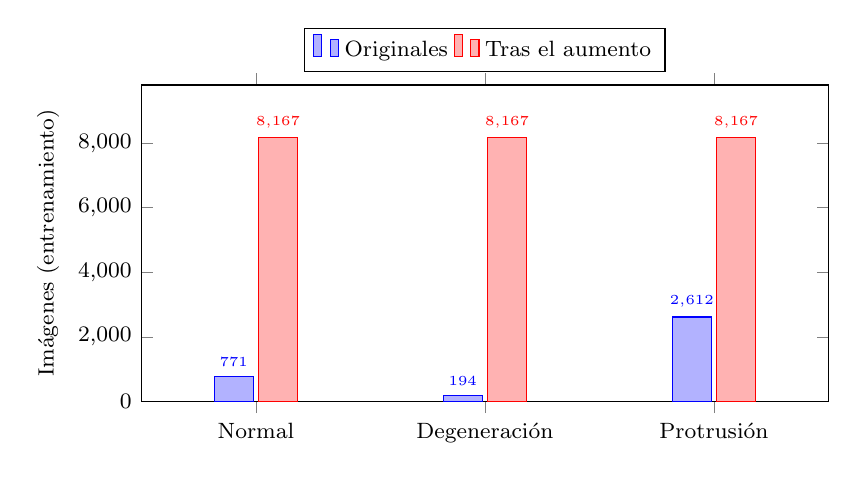
\begin{tikzpicture}
\begin{axis}[
  ybar, bar width=14pt, width=0.85\linewidth, height=5.6cm,
  symbolic x coords={Normal,Degeneración,Protrusión}, xtick=data,
  ymin=0, ymax=9800, ylabel={Imágenes (entrenamiento)},
  enlarge x limits=0.25, legend style={at={(0.5,1.04)},anchor=south,legend columns=2,font=\footnotesize},
  nodes near coords, every node near coord/.append style={font=\tiny},
  tick label style={font=\footnotesize}, ylabel style={font=\footnotesize}]
\addplot coordinates {(Normal,771) (Degeneración,194) (Protrusión,2612)};
\addplot coordinates {(Normal,8167) (Degeneración,8167) (Protrusión,8167)};
\legend{Originales, Tras el aumento}
\end{axis}
\end{tikzpicture}
\caption{Balance por conteo en entrenamiento: ROI originales y total tras el aumento.}
\label{fig:balance}
\end{figure}

\paragraph{Trazabilidad.} Cada archivo se llama \arch{T2_TSE_SAG__0188_008_L4-L5__orig.png} (original) o \arch{..._aug012.png} (copia), con paciente, corte y nivel. El manifiesto \arch{manifest_35k.csv} registra, para cada una de las 35\,007 imágenes, su partición, clase, paciente, nivel, ROI original, revisor y, en las copias, los parámetros exactos (semilla, ángulo, zoom, desplazamientos, contraste y brillo); \arch{split_pacientes.csv} guarda la partición de cada paciente. Las copias respetan los rangos declarados (ángulo entre $-8^{\circ}$ y $8^{\circ}$, zoom entre 0,90 y 1,10, contraste entre 0,90 y 1,10).

\paragraph{Verificaciones.} El script comprueba que (i) los conjuntos de pacientes de las tres particiones son disjuntos, (ii) toda copia está en la misma partición que su original, (iii) los nombres de archivo son únicos, (iv) todo PNG está íntegro y (v) el total supera los 35\,000.

\subsection{Balance de clases y sesgo por nivel}
\label{sec:balance}
El balance de 1/3 por clase es \emph{por conteo}, no por originales. Entre los 5\,123 ROI originales, la Protrusión es el 73,0\,\% (3\,738), Normal el 21,6\,\% (1\,105) y Degeneración el 5,5\,\% (280); un clasificador que siempre dijera Protrusión acertaría cerca del 73\,\%. Las copias igualan la contribución de cada clase al entrenamiento, pero no añaden anatomía nueva: el tamaño efectivo del dataset es el número de pacientes (399), y la Degeneración, repetida unas 42 veces, solo tiene 42 originales en la partición de prueba, lo que deja un margen de error amplio en su recall. Para que las métricas no se inflen con copias casi idénticas, los resultados principales se calculan sobre los \textbf{originales} de la partición de prueba, y el conjunto completo se reporta aparte. Además, un modelo entrenado con prior uniforme tiende a sobrepredecir las clases raras en la población real.

\begin{table}[t]
\centering\small
\caption{ROI originales elegibles por nivel y clase.}
\label{tab:nivel}
\begin{tabular}{lrrrrr}
\toprule
Nivel & Normal & Degeneración & Protrusión & Total & \% Protrusión \\
\midrule
L1-L2 & 505 & 121 & 401    & 1\,027 & 39,0 \\
L2-L3 & 383 & 94  & 550    & 1\,027 & 53,6 \\
L3-L4 & 172 & 44  & 811    & 1\,027 & 79,0 \\
L4-L5 & 15  & 5   & 1\,005 & 1\,025 & 98,0 \\
L5-S1 & 30  & 16  & 971    & 1\,017 & 95,5 \\
\bottomrule
\end{tabular}
\end{table}

La Tabla~\ref{tab:nivel} muestra un sesgo importante: casi toda la patología se concentra en L4-L5 y L5-S1. Un clasificador que solo adivinara la clase más frecuente de cada nivel acertaría 3\,842 de 5\,123 ROI (75,0\,\%), de modo que el nivel podría actuar como atajo. Por ello los resultados se reportan también por nivel. Esto relativiza cualquier umbral de exactitud: un 95\,\% medido sobre estas etiquetas mide acuerdo con etiquetas de estudiantes y puede alcanzarse en parte por el atajo, y cifras internas altas suelen bajar al evaluar con datos externos \cite{yi2023}. Por eso se acompaña la exactitud con F1 macro y recall por clase, que además es lo que justifica el uso de F1 con clases desbalanceadas \cite{alkubaisi2022}.

\subsection{Viabilidad del dataset}
\begin{itemize}
  \item \textbf{Disponibilidad y licencia.} Los datos son públicos y los scripts reproducen el procesamiento a partir de ellos. Las imágenes del dataset construido no se suben al repositorio: se distribuyen como un archivo comprimido de 405~MB y el repositorio guarda sus manifiestos.
  \item \textbf{Tamaño.} Cumple el requisito de más de 35\,000 registros. El contenido informativo real es menor: 5\,123 ROI de 399 pacientes, con 280 originales de Degeneración.
  \item \textbf{Balance.} Equilibrado por conteo entre las tres clases y en cada partición; desbalanceado en originales y por nivel (Secciones~\ref{sec:aumento} y~\ref{sec:balance}).
  \item \textbf{Reproducibilidad.} Semilla única (42), manifiesto por imagen y verificaciones automáticas.
  \item \textbf{Cómputo.} Los cuatro modelos se entrenaron con este mismo dataset en una GPU de consumo (RTX 3060~Ti), lo que indica que el tamaño es manejable con recursos modestos.
\end{itemize}

\subsection{Limitaciones}
(1) Las etiquetas son de estudiantes, sin radiólogo, con apoyo de un modelo, y no se midió el acuerdo entre anotadores. (2) Solo hay plano sagital; Hernia y Abombamiento no son separables y se fusionaron después de ver los datos. (3) Un único equipo de resonancia de 1,5~T, sin diversidad de escáner. (4) El tamaño efectivo son 399 pacientes; las copias no aportan anatomía nueva. (5) Degeneración cuenta con pocos pacientes (81, 17 y 22 en las tres particiones). (6) Sesgo por nivel y prior uniforme (Sección~\ref{sec:balance}). (7) Con el identificador de paciente vacío no puede descartarse la presencia de un mismo paciente en dos carpetas. (8) El conjunto es una herramienta académica, no diagnóstica.

% Paquetes requeridos: graphicx, booktabs, xcolor, tikz (+ calc no), pgfplots, caption
% Figuras: guia_visual_5rois.png vive en docs/guias/ (ver \graphicspath en el archivo principal)
% Las cifras salen de data/processed/etiquetado/etiquetas_revisadas.csv,
% data/processed/dataset_35k/manifest_35k.csv y de los scripts de scripts/.
% Todo lo que no se pudo verificar se marca con \pendiente{...} (se ve en rojo).
% =====================================================================
\providecommand{\pendiente}[1]{\textcolor{red}{\textbf{[PENDIENTE: #1]}}}
\providecommand{\arch}[1]{\texttt{\detokenize{#1}}}

\section{Preparación del dataset}
\label{sec:dataset}

Esta sección describe, en orden, cómo se pasó del conjunto público original a los 35\,007 recortes (ROI) con los que se entrenaron y compararon los cuatro modelos. La Figura~\ref{fig:flujo} resume el flujo y el número de elementos que pasan por cada etapa. Todas las cifras proceden de los archivos versionados del repositorio; lo que no pudo verificarse se señala como pendiente.

\begin{figure}[t]
\centering
\begin{tikzpicture}[
  box/.style={draw, rounded corners=2pt, align=left, text width=0.60\linewidth, inner sep=3pt, font=\footnotesize},
  num/.style={align=left, text width=0.30\linewidth, font=\footnotesize\bfseries},
  arrow/.style={-{Stealth[length=2mm]}, thick},
  node distance=4.2mm]
  \node[box] (a) {1. Conjunto público (Mendeley), archivos \texttt{.IMA}};
  \node[num, right=3mm of a] {575 carpetas, $\approx$48\,000 archivos};
  \node[box, below=of a] (b) {2. Descarte de series inútiles y conservación de T2 sagital};
  \node[num, right=3mm of b] {solo T2 sagital};
  \node[box, below=of b] (c) {3. Conversión DICOM$\to$PNG y limpieza manual de cortes};
  \node[num, right=3mm of c] {1\,086 cortes, 414 pacientes};
  \node[box, below=of c] (d) {4. Recorte L1--S1 y detección de discos (ROI 128$\times$128)};
  \node[num, right=3mm of d] {5\,385 ROI};
  \node[box, below=of d] (e) {5. Preetiquetado, revisión humana (A/B) y exclusiones};
  \node[num, right=3mm of e] {5\,123 ROI, 399 pacientes};
  \node[box, below=of e] (f) {6. División por paciente 70/15/15};
  \node[num, right=3mm of f] {279 / 60 / 60 pacientes};
  \node[box, below=of f] (g) {7. Aumento dentro de cada partición (balance por conteo)};
  \node[num, right=3mm of g] {35\,007 imágenes};
  \foreach \i/\j in {a/b,b/c,c/d,d/e,e/f,f/g} \draw[arrow] (\i) -- (\j);
\end{tikzpicture}
\caption{Flujo de preparación del dataset y número de elementos en cada etapa.}
\label{fig:flujo}
\end{figure}

\subsection{Origen de los datos}
Se usó el \emph{Lumbar Spine MRI Dataset} (Mendeley Data) \cite{sudirman2019}, el mismo conjunto público empleado en trabajos previos sobre clasificación de hernia discal \cite{sari2024}. Los estudios se adquirieron con un único equipo, un Siemens MAGNETOM Essenza de 1,5~T, y se distribuyen como archivos DICOM con extensión \arch{.IMA}, en una carpeta por paciente. Los cortes tienen un tamaño de píxel de 0,729~mm, un grosor de 4~mm y una separación entre centros de 4,8~mm. El campo \texttt{PatientID} está vacío en todo el corpus y el repositorio solo conserva identificadores de estudio y de serie (los campos de nombre, nacimiento y fecha están vacíos en \arch{meta_dicom_por_slice.csv}). El conjunto descargado contenía 575 carpetas de pacientes. Se eliminaron las que, en lugar de resonancia lumbar, contenían estudios del segmento cervical o de rodillas, y las lumbares con aberraciones o manchas que habrían introducido ruido en los modelos. Tras esa depuración quedaron 414 pacientes con cortes útiles y, tras las exclusiones de calidad de los ROI (Sección~\ref{sec:roi}), los \textbf{399 pacientes} del dataset final. Cada una de las 414 carpetas restantes corresponde a un \texttt{StudyInstanceUID} distinto y no se repite ningún \texttt{StudyTime}; no hay evidencia de pacientes duplicados, aunque con el identificador vacío no puede descartarse del todo.
% VERIFICAR: el sitio de Mendeley describe 515 pacientes; el equipo reporta 575 carpetas descargadas.

\subsection{Depuración de la fuente}
La descarga inicial contenía cerca de 48\,000 registros en formato \arch{.IMA}. Cada paciente trae varias series; solo una parte sirve para este problema. La Tabla~\ref{tab:descartes} lista lo que se descartó y por qué.

\begin{table}[t]
\centering\small
\caption{Series descartadas de cada estudio y motivo.}
\label{tab:descartes}
\begin{tabular}{p{0.30\linewidth}p{0.60\linewidth}}
\toprule
Serie & Motivo del descarte \\
\midrule
\arch{LOCALIZER_0001} & Localizadores de muy baja resolución usados por el técnico para calibrar la mesa y posicionar al paciente; no aportan información anatómica ni de textura. \\
\arch{POSDISP_[4]_T2_TSE_TRA_...} & Vistas sagitales con líneas blancas superpuestas (\emph{overlays}) que marcan los planos transversales; ese artefacto distorsiona descriptores de textura (GLCM/LBP) y confunde a las redes. \\
\arch{T1_TSE_SAG_...}, \arch{T1_TSE_TRA_...} & En T1 la grasa es brillante y el líquido oscuro, de modo que no permite evaluar la hidratación del disco (base de la escala de Pfirrmann); además, mezclar T1 y T2 altera los rangos de brillo. \\
\arch{T2_TSE_TRA_...} (axial) & Cortes axiales fragmentados en lotes de 3 a 5 por nivel; exigirían un emparejamiento espacial adicional por disco, mientras que el plano sagital cubre L1--S1 en una sola imagen. Se deja para una fase futura. \\
\bottomrule
\end{tabular}
\end{table}

El proceso se hizo en cuatro pasos, cada uno con su script (carpeta \arch{scripts/preprocesamiento/}):
\begin{enumerate}
  \item \arch{ingestion.py} recorre las carpetas de pacientes y copia solo las imágenes T2 sagitales, identificadas por el nombre de la serie.
  \item \arch{limpiar_slices.py} conserva el 40\,\% central del volumen sagital (se descarta el 30\,\% inicial y el 30\,\% final), donde el canal medular y la región L1--S1 son visibles.
  \item \arch{convertidor_dcm_a_png.py} convierte a PNG de 8 bits con una sola escala por serie: percentiles 1 y 99,5 calculados sobre los píxeles de tejido. Se decidió no aplicar CLAHE ni otro realce, para no alterar la señal relativa del T2 que sustenta el criterio diagnóstico.
  \item Depuración manual de los PNG: algunos pacientes tenían estudios del segmento cervical o de rodillas, y otros cortes T2 sagitales quedaban oscuros o con aberraciones; se eliminaron.
\end{enumerate}
Tras esta depuración quedaron \textbf{1\,086 cortes sagitales de 414 pacientes} (2,6 cortes por paciente en promedio; entre 1 y 6).

\subsection{Recorte de la región lumbar y de los ROI por disco}
\label{sec:roi}
\paragraph{Recorte L1--S1.} Con \arch{aplicar_recortes.py} se recortó cada corte en altura para abarcar principalmente L1--S1, replicando por \emph{template matching} unos recortes manuales previos (mediana de la puntuación de coincidencia 0,9996; solo el corte 0547\_008 quedó por debajo de 0,99). El recorte se extendió 60~px hacia arriba y hacia abajo hasta el borde de la imagen; con ello el relleno necesario en L1-L2 bajó de 779 de 1\,080 recortes (72\,\%) a cero.

\paragraph{Detector de discos.} Para localizar los discos se entrenó un detector con un conjunto propio en Roboflow (proyecto \emph{Intervertebral Disks}, versión~1): 100 cortes (70 de entrenamiento, 20 de validación y 10 de prueba), con orientación automática (\emph{auto-orient}) y reescalado a 640$\times$640 con bordes negros, sin aumento de datos en Roboflow. Las cinco clases del detector son los niveles L1-L2 a L5-S1. Se ajustó un YOLOv8n de detección de cajas (\arch{yolov8n.pt}) durante 50 épocas, con paciencia 30, lote 16, imagen de 640~px y semilla 42; el aumento en línea de Ultralytics (mosaico, escala, traslación, brillo) es el predeterminado, con reflexión horizontal. La mejor época en validación fue la 49. El detector solo ubica el nivel del disco; no clasifica patología. La Tabla~\ref{tab:detector} resume su desempeño con el umbral de uso (confianza 0,35).

\begin{table}[t]
\centering\small
\caption{Desempeño del detector de discos (corrida \arch{detector_discos_v1_s42}).}
\label{tab:detector}
\begin{tabular}{lrrrrrrr}
\toprule
Partición & Cortes & Precisión & Recall & mAP50 & mAP50-95 & Cortes con 5 niveles & IoU medio \\
\midrule
Validación & 20 & 0,922 & 0,964 & 0,962 & 0,663 & 95\,\% & 0,819 \\
Prueba     & 10 & 0,983 & 0,994 & 0,995 & 0,691 & 100\,\% & 0,843 \\
\bottomrule
\end{tabular}
\end{table}

El nivel más difícil es L1-L2 (en validación: precisión 0,839, recall 0,820 y IoU 0,74); los demás tienen recall de 1,0. Con solo 20 y 10 cortes, un corte mueve varios puntos porcentuales; es una sola corrida con una sola semilla, y la época se eligió con la validación, por lo que sus cifras están algo infladas.

\paragraph{Extracción del ROI.} Con \arch{autocrop_rois.py} se detecta sobre el recorte y se extrae el parche sobre el PNG completo, sumando el desplazamiento. La caja se amplía (margen posterior 0,40, anterior 0,10 y vertical 0,50), se hace cuadrada y se guarda a 128$\times$128~px, una por nivel (L1-L2, L2-L3, L3-L4, L4-L5 y L5-S1). Cada recorte queda registrado en \arch{roi_log.csv} con su caja, su ordenada central, su confianza y el relleno por lado. El resultado fueron \textbf{5\,385 ROI}. El margen anterior de L5-S1 se probó en 0,20 frente a 0,10 y la ganancia fue marginal, por lo que se mantuvo 0,10. La Figura~\ref{fig:rois} muestra los cinco ROI de un corte.

\begin{figure}[t]
\centering
\includegraphics[width=0.9\linewidth]{guia_visual_5rois.png}
\caption{Los cinco ROI (L1-L2 a L5-S1) de un corte sagital T2. \pendiente{confirmar que es la figura que se quiere en el informe o sustituirla por un montaje propio con las cajas del detector}}
\label{fig:rois}
\end{figure}

\paragraph{Exclusiones por calidad.} Se aplicaron reglas objetivas sobre \arch{roi_log.csv} (función \arch{elegibles()} de \arch{scripts/build_dataset.py}): se descarta el corte completo si falta algún nivel, si dos niveles adyacentes se solapan (IoU $>0{,}5$) o si el orden vertical de los centros no crece de L1-L2 a L5-S1; además se excluyen el paciente 0456, el corte 0547\_008 y los ROI con confianza del detector menor que 0,5. En total se excluyeron \textbf{262 ROI}, que afectan a 48 pacientes; 15 pacientes quedaron fuera por completo. Así, los 5\,385 ROI etiquetados quedan en \textbf{5\,123 ROI de 399 pacientes}; los 15 pacientes restantes (de los 414) no conservaron ningún ROI elegible. De los ROI excluidos, 207 eran Protrusión, 38 Normal y 17 Degeneración.

\subsection{Anotación y retiquetado}
\paragraph{Clases.} La guía de anotación (\arch{docs/guias/guia_anotacion_4_clases.md}) define cuatro clases nominales: Normal, Degeneración, Abombamiento y Hernia. Cuando coinciden varias, se aplica la prioridad Hernia $>$ Abombamiento $>$ Degeneración $>$ Normal, que solo sirve para desempatar el etiquetado y no es un orden de gravedad. La guía recoge criterios de uso común y no está validada por un radiólogo. Las etiquetas las asignaron estudiantes, sin radiólogo.

\paragraph{Fusión a tres clases.} En la primera corrida del clasificador semilla, con las cuatro clases (60 imágenes de validación) la exactitud fue 0,65 (IC 95\,\%: 0,52--0,76) y 10 de los 20 errores fueron confusiones Hernia--Abombamiento. Sin un corte axial, la extensión del abultamiento sobre la circunferencia del disco, que es lo que separa ambas entidades en la nomenclatura de consenso \cite{fardon2014}, no puede medirse. Por eso Hernia y Abombamiento se fusionaron en \textbf{Protrusión}, quedando tres clases: Normal, Degeneración discal y Protrusión. Otros autores también reportan confusión entre abultamiento y protrusión \cite{gao2025}. La fusión es una decisión posterior a ver los datos (\emph{post hoc}) y se declara así.

\paragraph{Preetiquetado y revisión.} Etiquetar 5\,385 ROI a mano desde cero era inviable en el plazo, así que se siguió un esquema de aprendizaje activo. Primero se etiquetó a mano una semilla en Roboflow (proyecto \emph{deepspine-seed-350-cls}); su versión~3, la usada para el preetiquetado final, tiene 719 imágenes de entrenamiento y 84 de validación (24 Degeneración, 30 Normal y 30 Protrusión). Con ella se entrenó un clasificador pequeño, YOLOv8s-cls (entrada 224$\times$224, hasta 60 épocas, paciencia 15, lote 32, semilla 42; cuaderno \arch{entrenamiento_clasificador_semilla_v3.ipynb}). En validación alcanzó una exactitud de 0,833 (IC 95\,\%: 0,739--0,898) y un F1 de 0,784 en Degeneración, 0,852 en Normal y 0,857 en Protrusión; con solo 84 imágenes de validación estas cifras son una guía y no una garantía. El modelo preetiquetó los 5\,385 ROI con su clase y su confianza (media 0,946; mediana 1,0) y marcó 2\,265 (42,1\,\%) para revisión prioritaria: 1\,881 por predecir una clase rara (Protrusión) y el resto por confianza menor que 0,7, por margen menor que 0,2 entre las dos primeras clases, o por combinación de motivos.

Después, todos los ROI pasaron por revisión humana en dos grupos, A y B, de 2\,693 y 2\,692 ROI respectivamente. La clase final es la decisión humana. De los 5\,385 ROI, 3\,366 (62,5\,\%) conservaron la clase del modelo y \textbf{2\,019 (37,5\,\%) fueron corregidos}. La Tabla~\ref{tab:reetiquetado} muestra cómo se reorganizó el dataset.

\begin{table}[t]
\centering\small
\caption{Clase propuesta por el preetiquetador frente a la clase final tras la revisión humana (5\,385 ROI).}
\label{tab:reetiquetado}
\begin{tabular}{lrrrrr}
\toprule
 & \multicolumn{3}{c}{Clase final} & & \\
\cmidrule(lr){2-4}
Predicha & Normal & Degeneración & Protrusión & Total & Corregidas \\
\midrule
Normal       & 1\,086 & 32  & 1\,387 & 2\,505 & 56,6\,\% \\
Degeneración & 51     & 256 & 534    & 841    & 69,6\,\% \\
Protrusión   & 6      & 9   & 2\,024 & 2\,039 & 0,7\,\% \\
\midrule
Total final  & 1\,143 & 297 & 3\,945 & 5\,385 & 37,5\,\% \\
\bottomrule
\end{tabular}
\end{table}

La lectura de la Tabla~\ref{tab:reetiquetado} es clara: el preetiquetador, entrenado con una semilla balanceada, \emph{subestimó} la Protrusión. De los 3\,945 ROI de Protrusión finales, 1\,921 (48,7\,\%) llegaron como Normal o Degeneración, mientras que casi nadie de lo que predijo como Protrusión cambió (15 de 2\,039). Dicho de otro modo, la revisión humana fue lo que fijó la distribución de clases del dataset, no el modelo, y la distribución real está muy desbalanceada (Sección~\ref{sec:balance}).

\paragraph{Fiabilidad de las etiquetas.} Cada ROI fue revisado por una sola persona (A o B); 408 de los 414 pacientes tienen ROI revisados por ambos, pero no hay ROI doble. En consecuencia \textbf{no puede calcularse el coeficiente kappa entre anotadores}. Sí se observan diferencias de criterio: A etiquetó Degeneración en el 6,9\,\% de sus ROI y B en el 4,1\,\%, y corrigió el 35,3\,\% frente al 39,7\,\% de B. No es posible separar cuánto de esa diferencia es criterio y cuánto es composición de la muestra.

\subsection{División por paciente}
\label{sec:split}
Cada paciente aporta unos 13 ROI (5\,123/399) de cortes vecinos casi idénticos. Si se dividiera por imagen, un paciente quedaría repartido entre entrenamiento y prueba y el modelo podría reconocer al paciente en lugar de la patología, inflando las métricas (fuga de datos) \cite{brunekreef2024,rumala2023}. Por eso \textbf{cada paciente va entero a una sola partición}.

El reparto es 70/15/15 por pacientes, con semilla 42. El script prueba 20\,000 repartos aleatorios y conserva el que mejor mantiene, en las tres particiones, la proporción de cada clase (con peso triple) y de cada nivel. Se eligieron tres particiones porque la validación sirve para decidir (época, hiperparámetros, umbrales) y la prueba para medir una sola vez al final, con todo ya decidido. La Tabla~\ref{tab:split} muestra el resultado.

\begin{table}[t]
\centering\small
\caption{División por paciente y ROI originales por clase.}
\label{tab:split}
\begin{tabular}{lrrrrrr}
\toprule
Partición & Pacientes & Normal & Degeneración & Protrusión & ROI & \% ROI \\
\midrule
Entrenamiento & 279 & 771   & 194 & 2\,612 & 3\,577 & 69,8 \\
Validación    & 60  & 170   & 44  & 564    & 778    & 15,2 \\
Prueba        & 60  & 164   & 42  & 562    & 768    & 15,0 \\
\midrule
Total         & 399 & 1\,105 & 280 & 3\,738 & 5\,123 & 100 \\
\bottomrule
\end{tabular}
\end{table}

La intersección de pacientes entre particiones es vacía y se comprueba con aserciones en el script. Los pacientes con al menos un ROI de Degeneración son 81, 17 y 22 en entrenamiento, validación y prueba. La docente aceptó esta división, y los 35\,007 registros que exige la rúbrica son las 35\,007 imágenes del dataset.

\subsection{Construcción del dataset de 35\,007 imágenes}
\label{sec:aumento}
La rúbrica exige un dataset balanceado con más de 35\,000 registros. Como los ROI originales son 5\,123, se recurrió a aumento de datos, siempre \emph{después} de dividir y \emph{dentro} de cada partición, para que ninguna copia cruce de partición. La cantidad de copias por ROI se calcula para que cada clase alcance la misma meta por partición: 8\,167 imágenes por clase en entrenamiento y 1\,751 en validación y en prueba, es decir 35\,007 en total.

\paragraph{Transformaciones.} Rotación de $\pm 8^{\circ}$, desplazamiento de hasta $\pm 8\,\%$ del tamaño, zoom entre 0,90 y 1,10, y brillo y contraste de $\pm 10\,\%$, con reflejo en los bordes. No se usan reflexiones (el eje anterior--posterior tiene significado anatómico), deformación elástica ni realce. Cada copia se genera con una semilla derivada de un hash (SHA-256) del nombre del ROI, la semilla global y el índice de la copia, por lo que el proceso es determinista y reproducible.

\begin{table}[t]
\centering\small
\caption{Imágenes finales por partición y clase (mismo número por clase en cada partición), ROI originales y copias por original.}
\label{tab:35k}
\begin{tabular}{llrrrr}
\toprule
Partición & Clase & Originales & Aumentadas & Total & Copias por original \\
\midrule
Entrenamiento & Normal       & 771    & 7\,396 & 8\,167 & 10,6 \\
              & Degeneración & 194    & 7\,973 & 8\,167 & 42,1 \\
              & Protrusión   & 2\,612 & 5\,555 & 8\,167 & 3,1  \\
Validación    & Normal       & 170    & 1\,581 & 1\,751 & 10,3 \\
              & Degeneración & 44     & 1\,707 & 1\,751 & 39,8 \\
              & Protrusión   & 564    & 1\,187 & 1\,751 & 3,1  \\
Prueba        & Normal       & 164    & 1\,587 & 1\,751 & 10,7 \\
              & Degeneración & 42     & 1\,709 & 1\,751 & 41,7 \\
              & Protrusión   & 562    & 1\,189 & 1\,751 & 3,1  \\
\midrule
Total         &              & 5\,123 & 29\,884 & 35\,007 & \\
\bottomrule
\end{tabular}
\end{table}

\begin{figure}[t]
\centering
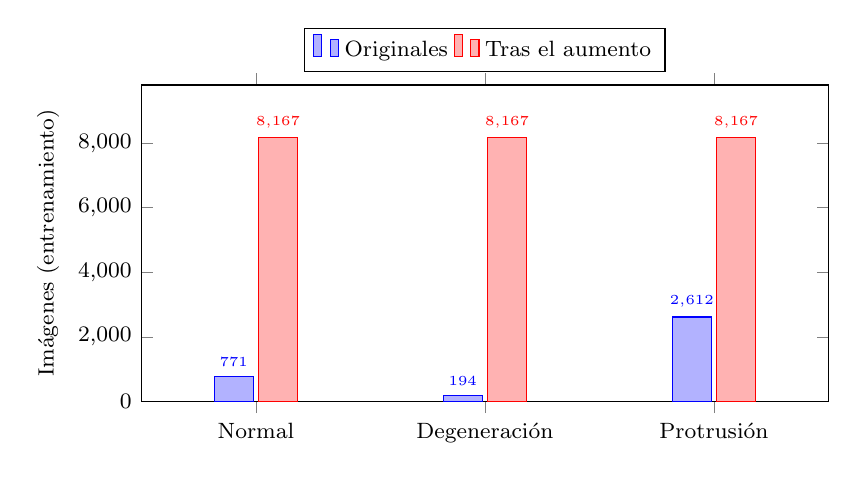
\begin{tikzpicture}
\begin{axis}[
  ybar, bar width=14pt, width=0.85\linewidth, height=5.6cm,
  symbolic x coords={Normal,Degeneración,Protrusión}, xtick=data,
  ymin=0, ymax=9800, ylabel={Imágenes (entrenamiento)},
  enlarge x limits=0.25, legend style={at={(0.5,1.04)},anchor=south,legend columns=2,font=\footnotesize},
  nodes near coords, every node near coord/.append style={font=\tiny},
  tick label style={font=\footnotesize}, ylabel style={font=\footnotesize}]
\addplot coordinates {(Normal,771) (Degeneración,194) (Protrusión,2612)};
\addplot coordinates {(Normal,8167) (Degeneración,8167) (Protrusión,8167)};
\legend{Originales, Tras el aumento}
\end{axis}
\end{tikzpicture}
\caption{Balance por conteo en entrenamiento: ROI originales y total tras el aumento.}
\label{fig:balance}
\end{figure}

\paragraph{Trazabilidad.} Cada archivo se llama \arch{T2_TSE_SAG__0188_008_L4-L5__orig.png} (original) o \arch{..._aug012.png} (copia), con paciente, corte y nivel. El manifiesto \arch{manifest_35k.csv} registra, para cada una de las 35\,007 imágenes, su partición, clase, paciente, nivel, ROI original, revisor y, en las copias, los parámetros exactos (semilla, ángulo, zoom, desplazamientos, contraste y brillo); \arch{split_pacientes.csv} guarda la partición de cada paciente. Las copias respetan los rangos declarados (ángulo entre $-8^{\circ}$ y $8^{\circ}$, zoom entre 0,90 y 1,10, contraste entre 0,90 y 1,10).

\paragraph{Verificaciones.} El script comprueba que (i) los conjuntos de pacientes de las tres particiones son disjuntos, (ii) toda copia está en la misma partición que su original, (iii) los nombres de archivo son únicos, (iv) todo PNG está íntegro y (v) el total supera los 35\,000.

\subsection{Balance de clases y sesgo por nivel}
\label{sec:balance}
El balance de 1/3 por clase es \emph{por conteo}, no por originales. Entre los 5\,123 ROI originales, la Protrusión es el 73,0\,\% (3\,738), Normal el 21,6\,\% (1\,105) y Degeneración el 5,5\,\% (280); un clasificador que siempre dijera Protrusión acertaría cerca del 73\,\%. Las copias igualan la contribución de cada clase al entrenamiento, pero no añaden anatomía nueva: el tamaño efectivo del dataset es el número de pacientes (399), y la Degeneración, repetida unas 42 veces, solo tiene 42 originales en la partición de prueba, lo que deja un margen de error amplio en su recall. Para que las métricas no se inflen con copias casi idénticas, los resultados principales se calculan sobre los \textbf{originales} de la partición de prueba, y el conjunto completo se reporta aparte. Además, un modelo entrenado con prior uniforme tiende a sobrepredecir las clases raras en la población real.

\begin{table}[t]
\centering\small
\caption{ROI originales elegibles por nivel y clase.}
\label{tab:nivel}
\begin{tabular}{lrrrrr}
\toprule
Nivel & Normal & Degeneración & Protrusión & Total & \% Protrusión \\
\midrule
L1-L2 & 505 & 121 & 401    & 1\,027 & 39,0 \\
L2-L3 & 383 & 94  & 550    & 1\,027 & 53,6 \\
L3-L4 & 172 & 44  & 811    & 1\,027 & 79,0 \\
L4-L5 & 15  & 5   & 1\,005 & 1\,025 & 98,0 \\
L5-S1 & 30  & 16  & 971    & 1\,017 & 95,5 \\
\bottomrule
\end{tabular}
\end{table}

La Tabla~\ref{tab:nivel} muestra un sesgo importante: casi toda la patología se concentra en L4-L5 y L5-S1. Un clasificador que solo adivinara la clase más frecuente de cada nivel acertaría 3\,842 de 5\,123 ROI (75,0\,\%), de modo que el nivel podría actuar como atajo. Por ello los resultados se reportan también por nivel. Esto relativiza cualquier umbral de exactitud: un 95\,\% medido sobre estas etiquetas mide acuerdo con etiquetas de estudiantes y puede alcanzarse en parte por el atajo, y cifras internas altas suelen bajar al evaluar con datos externos \cite{yi2023}. Por eso se acompaña la exactitud con F1 macro y recall por clase, que además es lo que justifica el uso de F1 con clases desbalanceadas \cite{alkubaisi2022}.

\subsection{Viabilidad del dataset}
\begin{itemize}
  \item \textbf{Disponibilidad y licencia.} Los datos son públicos y los scripts reproducen el procesamiento a partir de ellos. Las imágenes del dataset construido no se suben al repositorio: se distribuyen como un archivo comprimido de 405~MB y el repositorio guarda sus manifiestos.
  \item \textbf{Tamaño.} Cumple el requisito de más de 35\,000 registros. El contenido informativo real es menor: 5\,123 ROI de 399 pacientes, con 280 originales de Degeneración.
  \item \textbf{Balance.} Equilibrado por conteo entre las tres clases y en cada partición; desbalanceado en originales y por nivel (Secciones~\ref{sec:aumento} y~\ref{sec:balance}).
  \item \textbf{Reproducibilidad.} Semilla única (42), manifiesto por imagen y verificaciones automáticas.
  \item \textbf{Cómputo.} Los cuatro modelos se entrenaron con este mismo dataset en una GPU de consumo (RTX 3060~Ti), lo que indica que el tamaño es manejable con recursos modestos.
\end{itemize}

\subsection{Limitaciones}
(1) Las etiquetas son de estudiantes, sin radiólogo, con apoyo de un modelo, y no se midió el acuerdo entre anotadores. (2) Solo hay plano sagital; Hernia y Abombamiento no son separables y se fusionaron después de ver los datos. (3) Un único equipo de resonancia de 1,5~T, sin diversidad de escáner. (4) El tamaño efectivo son 399 pacientes; las copias no aportan anatomía nueva. (5) Degeneración cuenta con pocos pacientes (81, 17 y 22 en las tres particiones). (6) Sesgo por nivel y prior uniforme (Sección~\ref{sec:balance}). (7) Con el identificador de paciente vacío no puede descartarse la presencia de un mismo paciente en dos carpetas. (8) El conjunto es una herramienta académica, no diagnóstica.

% Paquetes requeridos: graphicx, booktabs, xcolor, tikz (+ calc no), pgfplots, caption
% Figuras: guia_visual_5rois.png vive en docs/guias/ (ver \graphicspath en el archivo principal)
% Las cifras salen de data/processed/etiquetado/etiquetas_revisadas.csv,
% data/processed/dataset_35k/manifest_35k.csv y de los scripts de scripts/.
% Todo lo que no se pudo verificar se marca con \pendiente{...} (se ve en rojo).
% =====================================================================
\providecommand{\pendiente}[1]{\textcolor{red}{\textbf{[PENDIENTE: #1]}}}
\providecommand{\arch}[1]{\texttt{\detokenize{#1}}}

\section{Preparación del dataset}
\label{sec:dataset}

Esta sección describe, en orden, cómo se pasó del conjunto público original a los 35\,007 recortes (ROI) con los que se entrenaron y compararon los cuatro modelos. La Figura~\ref{fig:flujo} resume el flujo y el número de elementos que pasan por cada etapa. Todas las cifras proceden de los archivos versionados del repositorio; lo que no pudo verificarse se señala como pendiente.

\begin{figure}[t]
\centering
\begin{tikzpicture}[
  box/.style={draw, rounded corners=2pt, align=left, text width=0.60\linewidth, inner sep=3pt, font=\footnotesize},
  num/.style={align=left, text width=0.30\linewidth, font=\footnotesize\bfseries},
  arrow/.style={-{Stealth[length=2mm]}, thick},
  node distance=4.2mm]
  \node[box] (a) {1. Conjunto público (Mendeley), archivos \texttt{.IMA}};
  \node[num, right=3mm of a] {575 carpetas, $\approx$48\,000 archivos};
  \node[box, below=of a] (b) {2. Descarte de series inútiles y conservación de T2 sagital};
  \node[num, right=3mm of b] {solo T2 sagital};
  \node[box, below=of b] (c) {3. Conversión DICOM$\to$PNG y limpieza manual de cortes};
  \node[num, right=3mm of c] {1\,086 cortes, 414 pacientes};
  \node[box, below=of c] (d) {4. Recorte L1--S1 y detección de discos (ROI 128$\times$128)};
  \node[num, right=3mm of d] {5\,385 ROI};
  \node[box, below=of d] (e) {5. Preetiquetado, revisión humana (A/B) y exclusiones};
  \node[num, right=3mm of e] {5\,123 ROI, 399 pacientes};
  \node[box, below=of e] (f) {6. División por paciente 70/15/15};
  \node[num, right=3mm of f] {279 / 60 / 60 pacientes};
  \node[box, below=of f] (g) {7. Aumento dentro de cada partición (balance por conteo)};
  \node[num, right=3mm of g] {35\,007 imágenes};
  \foreach \i/\j in {a/b,b/c,c/d,d/e,e/f,f/g} \draw[arrow] (\i) -- (\j);
\end{tikzpicture}
\caption{Flujo de preparación del dataset y número de elementos en cada etapa.}
\label{fig:flujo}
\end{figure}

\subsection{Origen de los datos}
Se usó el \emph{Lumbar Spine MRI Dataset} (Mendeley Data) \cite{sudirman2019}, el mismo conjunto público empleado en trabajos previos sobre clasificación de hernia discal \cite{sari2024}. Los estudios se adquirieron con un único equipo, un Siemens MAGNETOM Essenza de 1,5~T, y se distribuyen como archivos DICOM con extensión \arch{.IMA}, en una carpeta por paciente. Los cortes tienen un tamaño de píxel de 0,729~mm, un grosor de 4~mm y una separación entre centros de 4,8~mm. El campo \texttt{PatientID} está vacío en todo el corpus y el repositorio solo conserva identificadores de estudio y de serie (los campos de nombre, nacimiento y fecha están vacíos en \arch{meta_dicom_por_slice.csv}). El conjunto descargado contenía 575 carpetas de pacientes. Se eliminaron las que, en lugar de resonancia lumbar, contenían estudios del segmento cervical o de rodillas, y las lumbares con aberraciones o manchas que habrían introducido ruido en los modelos. Tras esa depuración quedaron 414 pacientes con cortes útiles y, tras las exclusiones de calidad de los ROI (Sección~\ref{sec:roi}), los \textbf{399 pacientes} del dataset final. Cada una de las 414 carpetas restantes corresponde a un \texttt{StudyInstanceUID} distinto y no se repite ningún \texttt{StudyTime}; no hay evidencia de pacientes duplicados, aunque con el identificador vacío no puede descartarse del todo.
% VERIFICAR: el sitio de Mendeley describe 515 pacientes; el equipo reporta 575 carpetas descargadas.

\subsection{Depuración de la fuente}
La descarga inicial contenía cerca de 48\,000 registros en formato \arch{.IMA}. Cada paciente trae varias series; solo una parte sirve para este problema. La Tabla~\ref{tab:descartes} lista lo que se descartó y por qué.

\begin{table}[t]
\centering\small
\caption{Series descartadas de cada estudio y motivo.}
\label{tab:descartes}
\begin{tabular}{p{0.30\linewidth}p{0.60\linewidth}}
\toprule
Serie & Motivo del descarte \\
\midrule
\arch{LOCALIZER_0001} & Localizadores de muy baja resolución usados por el técnico para calibrar la mesa y posicionar al paciente; no aportan información anatómica ni de textura. \\
\arch{POSDISP_[4]_T2_TSE_TRA_...} & Vistas sagitales con líneas blancas superpuestas (\emph{overlays}) que marcan los planos transversales; ese artefacto distorsiona descriptores de textura (GLCM/LBP) y confunde a las redes. \\
\arch{T1_TSE_SAG_...}, \arch{T1_TSE_TRA_...} & En T1 la grasa es brillante y el líquido oscuro, de modo que no permite evaluar la hidratación del disco (base de la escala de Pfirrmann); además, mezclar T1 y T2 altera los rangos de brillo. \\
\arch{T2_TSE_TRA_...} (axial) & Cortes axiales fragmentados en lotes de 3 a 5 por nivel; exigirían un emparejamiento espacial adicional por disco, mientras que el plano sagital cubre L1--S1 en una sola imagen. Se deja para una fase futura. \\
\bottomrule
\end{tabular}
\end{table}

El proceso se hizo en cuatro pasos, cada uno con su script (carpeta \arch{scripts/preprocesamiento/}):
\begin{enumerate}
  \item \arch{ingestion.py} recorre las carpetas de pacientes y copia solo las imágenes T2 sagitales, identificadas por el nombre de la serie.
  \item \arch{limpiar_slices.py} conserva el 40\,\% central del volumen sagital (se descarta el 30\,\% inicial y el 30\,\% final), donde el canal medular y la región L1--S1 son visibles.
  \item \arch{convertidor_dcm_a_png.py} convierte a PNG de 8 bits con una sola escala por serie: percentiles 1 y 99,5 calculados sobre los píxeles de tejido. Se decidió no aplicar CLAHE ni otro realce, para no alterar la señal relativa del T2 que sustenta el criterio diagnóstico.
  \item Depuración manual de los PNG: algunos pacientes tenían estudios del segmento cervical o de rodillas, y otros cortes T2 sagitales quedaban oscuros o con aberraciones; se eliminaron.
\end{enumerate}
Tras esta depuración quedaron \textbf{1\,086 cortes sagitales de 414 pacientes} (2,6 cortes por paciente en promedio; entre 1 y 6).

\subsection{Recorte de la región lumbar y de los ROI por disco}
\label{sec:roi}
\paragraph{Recorte L1--S1.} Con \arch{aplicar_recortes.py} se recortó cada corte en altura para abarcar principalmente L1--S1, replicando por \emph{template matching} unos recortes manuales previos (mediana de la puntuación de coincidencia 0,9996; solo el corte 0547\_008 quedó por debajo de 0,99). El recorte se extendió 60~px hacia arriba y hacia abajo hasta el borde de la imagen; con ello el relleno necesario en L1-L2 bajó de 779 de 1\,080 recortes (72\,\%) a cero.

\paragraph{Detector de discos.} Para localizar los discos se entrenó un detector con un conjunto propio en Roboflow (proyecto \emph{Intervertebral Disks}, versión~1): 100 cortes (70 de entrenamiento, 20 de validación y 10 de prueba), con orientación automática (\emph{auto-orient}) y reescalado a 640$\times$640 con bordes negros, sin aumento de datos en Roboflow. Las cinco clases del detector son los niveles L1-L2 a L5-S1. Se ajustó un YOLOv8n de detección de cajas (\arch{yolov8n.pt}) durante 50 épocas, con paciencia 30, lote 16, imagen de 640~px y semilla 42; el aumento en línea de Ultralytics (mosaico, escala, traslación, brillo) es el predeterminado, con reflexión horizontal. La mejor época en validación fue la 49. El detector solo ubica el nivel del disco; no clasifica patología. La Tabla~\ref{tab:detector} resume su desempeño con el umbral de uso (confianza 0,35).

\begin{table}[t]
\centering\small
\caption{Desempeño del detector de discos (corrida \arch{detector_discos_v1_s42}).}
\label{tab:detector}
\begin{tabular}{lrrrrrrr}
\toprule
Partición & Cortes & Precisión & Recall & mAP50 & mAP50-95 & Cortes con 5 niveles & IoU medio \\
\midrule
Validación & 20 & 0,922 & 0,964 & 0,962 & 0,663 & 95\,\% & 0,819 \\
Prueba     & 10 & 0,983 & 0,994 & 0,995 & 0,691 & 100\,\% & 0,843 \\
\bottomrule
\end{tabular}
\end{table}

El nivel más difícil es L1-L2 (en validación: precisión 0,839, recall 0,820 y IoU 0,74); los demás tienen recall de 1,0. Con solo 20 y 10 cortes, un corte mueve varios puntos porcentuales; es una sola corrida con una sola semilla, y la época se eligió con la validación, por lo que sus cifras están algo infladas.

\paragraph{Extracción del ROI.} Con \arch{autocrop_rois.py} se detecta sobre el recorte y se extrae el parche sobre el PNG completo, sumando el desplazamiento. La caja se amplía (margen posterior 0,40, anterior 0,10 y vertical 0,50), se hace cuadrada y se guarda a 128$\times$128~px, una por nivel (L1-L2, L2-L3, L3-L4, L4-L5 y L5-S1). Cada recorte queda registrado en \arch{roi_log.csv} con su caja, su ordenada central, su confianza y el relleno por lado. El resultado fueron \textbf{5\,385 ROI}. El margen anterior de L5-S1 se probó en 0,20 frente a 0,10 y la ganancia fue marginal, por lo que se mantuvo 0,10. La Figura~\ref{fig:rois} muestra los cinco ROI de un corte.

\begin{figure}[t]
\centering
\includegraphics[width=0.9\linewidth]{guia_visual_5rois.png}
\caption{Los cinco ROI (L1-L2 a L5-S1) de un corte sagital T2. \pendiente{confirmar que es la figura que se quiere en el informe o sustituirla por un montaje propio con las cajas del detector}}
\label{fig:rois}
\end{figure}

\paragraph{Exclusiones por calidad.} Se aplicaron reglas objetivas sobre \arch{roi_log.csv} (función \arch{elegibles()} de \arch{scripts/build_dataset.py}): se descarta el corte completo si falta algún nivel, si dos niveles adyacentes se solapan (IoU $>0{,}5$) o si el orden vertical de los centros no crece de L1-L2 a L5-S1; además se excluyen el paciente 0456, el corte 0547\_008 y los ROI con confianza del detector menor que 0,5. En total se excluyeron \textbf{262 ROI}, que afectan a 48 pacientes; 15 pacientes quedaron fuera por completo. Así, los 5\,385 ROI etiquetados quedan en \textbf{5\,123 ROI de 399 pacientes}; los 15 pacientes restantes (de los 414) no conservaron ningún ROI elegible. De los ROI excluidos, 207 eran Protrusión, 38 Normal y 17 Degeneración.

\subsection{Anotación y retiquetado}
\paragraph{Clases.} La guía de anotación (\arch{docs/guias/guia_anotacion_4_clases.md}) define cuatro clases nominales: Normal, Degeneración, Abombamiento y Hernia. Cuando coinciden varias, se aplica la prioridad Hernia $>$ Abombamiento $>$ Degeneración $>$ Normal, que solo sirve para desempatar el etiquetado y no es un orden de gravedad. La guía recoge criterios de uso común y no está validada por un radiólogo. Las etiquetas las asignaron estudiantes, sin radiólogo.

\paragraph{Fusión a tres clases.} En la primera corrida del clasificador semilla, con las cuatro clases (60 imágenes de validación) la exactitud fue 0,65 (IC 95\,\%: 0,52--0,76) y 10 de los 20 errores fueron confusiones Hernia--Abombamiento. Sin un corte axial, la extensión del abultamiento sobre la circunferencia del disco, que es lo que separa ambas entidades en la nomenclatura de consenso \cite{fardon2014}, no puede medirse. Por eso Hernia y Abombamiento se fusionaron en \textbf{Protrusión}, quedando tres clases: Normal, Degeneración discal y Protrusión. Otros autores también reportan confusión entre abultamiento y protrusión \cite{gao2025}. La fusión es una decisión posterior a ver los datos (\emph{post hoc}) y se declara así.

\paragraph{Preetiquetado y revisión.} Etiquetar 5\,385 ROI a mano desde cero era inviable en el plazo, así que se siguió un esquema de aprendizaje activo. Primero se etiquetó a mano una semilla en Roboflow (proyecto \emph{deepspine-seed-350-cls}); su versión~3, la usada para el preetiquetado final, tiene 719 imágenes de entrenamiento y 84 de validación (24 Degeneración, 30 Normal y 30 Protrusión). Con ella se entrenó un clasificador pequeño, YOLOv8s-cls (entrada 224$\times$224, hasta 60 épocas, paciencia 15, lote 32, semilla 42; cuaderno \arch{entrenamiento_clasificador_semilla_v3.ipynb}). En validación alcanzó una exactitud de 0,833 (IC 95\,\%: 0,739--0,898) y un F1 de 0,784 en Degeneración, 0,852 en Normal y 0,857 en Protrusión; con solo 84 imágenes de validación estas cifras son una guía y no una garantía. El modelo preetiquetó los 5\,385 ROI con su clase y su confianza (media 0,946; mediana 1,0) y marcó 2\,265 (42,1\,\%) para revisión prioritaria: 1\,881 por predecir una clase rara (Protrusión) y el resto por confianza menor que 0,7, por margen menor que 0,2 entre las dos primeras clases, o por combinación de motivos.

Después, todos los ROI pasaron por revisión humana en dos grupos, A y B, de 2\,693 y 2\,692 ROI respectivamente. La clase final es la decisión humana. De los 5\,385 ROI, 3\,366 (62,5\,\%) conservaron la clase del modelo y \textbf{2\,019 (37,5\,\%) fueron corregidos}. La Tabla~\ref{tab:reetiquetado} muestra cómo se reorganizó el dataset.

\begin{table}[t]
\centering\small
\caption{Clase propuesta por el preetiquetador frente a la clase final tras la revisión humana (5\,385 ROI).}
\label{tab:reetiquetado}
\begin{tabular}{lrrrrr}
\toprule
 & \multicolumn{3}{c}{Clase final} & & \\
\cmidrule(lr){2-4}
Predicha & Normal & Degeneración & Protrusión & Total & Corregidas \\
\midrule
Normal       & 1\,086 & 32  & 1\,387 & 2\,505 & 56,6\,\% \\
Degeneración & 51     & 256 & 534    & 841    & 69,6\,\% \\
Protrusión   & 6      & 9   & 2\,024 & 2\,039 & 0,7\,\% \\
\midrule
Total final  & 1\,143 & 297 & 3\,945 & 5\,385 & 37,5\,\% \\
\bottomrule
\end{tabular}
\end{table}

La lectura de la Tabla~\ref{tab:reetiquetado} es clara: el preetiquetador, entrenado con una semilla balanceada, \emph{subestimó} la Protrusión. De los 3\,945 ROI de Protrusión finales, 1\,921 (48,7\,\%) llegaron como Normal o Degeneración, mientras que casi nadie de lo que predijo como Protrusión cambió (15 de 2\,039). Dicho de otro modo, la revisión humana fue lo que fijó la distribución de clases del dataset, no el modelo, y la distribución real está muy desbalanceada (Sección~\ref{sec:balance}).

\paragraph{Fiabilidad de las etiquetas.} Cada ROI fue revisado por una sola persona (A o B); 408 de los 414 pacientes tienen ROI revisados por ambos, pero no hay ROI doble. En consecuencia \textbf{no puede calcularse el coeficiente kappa entre anotadores}. Sí se observan diferencias de criterio: A etiquetó Degeneración en el 6,9\,\% de sus ROI y B en el 4,1\,\%, y corrigió el 35,3\,\% frente al 39,7\,\% de B. No es posible separar cuánto de esa diferencia es criterio y cuánto es composición de la muestra.

\subsection{División por paciente}
\label{sec:split}
Cada paciente aporta unos 13 ROI (5\,123/399) de cortes vecinos casi idénticos. Si se dividiera por imagen, un paciente quedaría repartido entre entrenamiento y prueba y el modelo podría reconocer al paciente en lugar de la patología, inflando las métricas (fuga de datos) \cite{brunekreef2024,rumala2023}. Por eso \textbf{cada paciente va entero a una sola partición}.

El reparto es 70/15/15 por pacientes, con semilla 42. El script prueba 20\,000 repartos aleatorios y conserva el que mejor mantiene, en las tres particiones, la proporción de cada clase (con peso triple) y de cada nivel. Se eligieron tres particiones porque la validación sirve para decidir (época, hiperparámetros, umbrales) y la prueba para medir una sola vez al final, con todo ya decidido. La Tabla~\ref{tab:split} muestra el resultado.

\begin{table}[t]
\centering\small
\caption{División por paciente y ROI originales por clase.}
\label{tab:split}
\begin{tabular}{lrrrrrr}
\toprule
Partición & Pacientes & Normal & Degeneración & Protrusión & ROI & \% ROI \\
\midrule
Entrenamiento & 279 & 771   & 194 & 2\,612 & 3\,577 & 69,8 \\
Validación    & 60  & 170   & 44  & 564    & 778    & 15,2 \\
Prueba        & 60  & 164   & 42  & 562    & 768    & 15,0 \\
\midrule
Total         & 399 & 1\,105 & 280 & 3\,738 & 5\,123 & 100 \\
\bottomrule
\end{tabular}
\end{table}

La intersección de pacientes entre particiones es vacía y se comprueba con aserciones en el script. Los pacientes con al menos un ROI de Degeneración son 81, 17 y 22 en entrenamiento, validación y prueba. La docente aceptó esta división, y los 35\,007 registros que exige la rúbrica son las 35\,007 imágenes del dataset.

\subsection{Construcción del dataset de 35\,007 imágenes}
\label{sec:aumento}
La rúbrica exige un dataset balanceado con más de 35\,000 registros. Como los ROI originales son 5\,123, se recurrió a aumento de datos, siempre \emph{después} de dividir y \emph{dentro} de cada partición, para que ninguna copia cruce de partición. La cantidad de copias por ROI se calcula para que cada clase alcance la misma meta por partición: 8\,167 imágenes por clase en entrenamiento y 1\,751 en validación y en prueba, es decir 35\,007 en total.

\paragraph{Transformaciones.} Rotación de $\pm 8^{\circ}$, desplazamiento de hasta $\pm 8\,\%$ del tamaño, zoom entre 0,90 y 1,10, y brillo y contraste de $\pm 10\,\%$, con reflejo en los bordes. No se usan reflexiones (el eje anterior--posterior tiene significado anatómico), deformación elástica ni realce. Cada copia se genera con una semilla derivada de un hash (SHA-256) del nombre del ROI, la semilla global y el índice de la copia, por lo que el proceso es determinista y reproducible.

\begin{table}[t]
\centering\small
\caption{Imágenes finales por partición y clase (mismo número por clase en cada partición), ROI originales y copias por original.}
\label{tab:35k}
\begin{tabular}{llrrrr}
\toprule
Partición & Clase & Originales & Aumentadas & Total & Copias por original \\
\midrule
Entrenamiento & Normal       & 771    & 7\,396 & 8\,167 & 10,6 \\
              & Degeneración & 194    & 7\,973 & 8\,167 & 42,1 \\
              & Protrusión   & 2\,612 & 5\,555 & 8\,167 & 3,1  \\
Validación    & Normal       & 170    & 1\,581 & 1\,751 & 10,3 \\
              & Degeneración & 44     & 1\,707 & 1\,751 & 39,8 \\
              & Protrusión   & 564    & 1\,187 & 1\,751 & 3,1  \\
Prueba        & Normal       & 164    & 1\,587 & 1\,751 & 10,7 \\
              & Degeneración & 42     & 1\,709 & 1\,751 & 41,7 \\
              & Protrusión   & 562    & 1\,189 & 1\,751 & 3,1  \\
\midrule
Total         &              & 5\,123 & 29\,884 & 35\,007 & \\
\bottomrule
\end{tabular}
\end{table}

\begin{figure}[t]
\centering
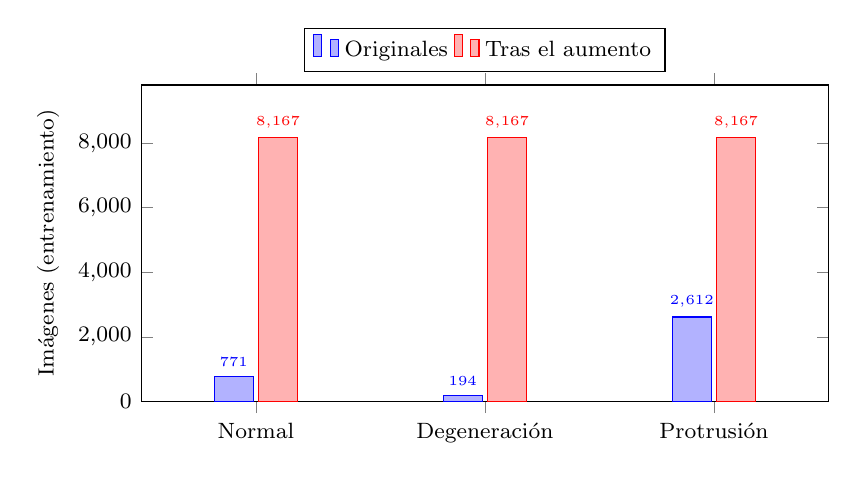
\begin{tikzpicture}
\begin{axis}[
  ybar, bar width=14pt, width=0.85\linewidth, height=5.6cm,
  symbolic x coords={Normal,Degeneración,Protrusión}, xtick=data,
  ymin=0, ymax=9800, ylabel={Imágenes (entrenamiento)},
  enlarge x limits=0.25, legend style={at={(0.5,1.04)},anchor=south,legend columns=2,font=\footnotesize},
  nodes near coords, every node near coord/.append style={font=\tiny},
  tick label style={font=\footnotesize}, ylabel style={font=\footnotesize}]
\addplot coordinates {(Normal,771) (Degeneración,194) (Protrusión,2612)};
\addplot coordinates {(Normal,8167) (Degeneración,8167) (Protrusión,8167)};
\legend{Originales, Tras el aumento}
\end{axis}
\end{tikzpicture}
\caption{Balance por conteo en entrenamiento: ROI originales y total tras el aumento.}
\label{fig:balance}
\end{figure}

\paragraph{Trazabilidad.} Cada archivo se llama \arch{T2_TSE_SAG__0188_008_L4-L5__orig.png} (original) o \arch{..._aug012.png} (copia), con paciente, corte y nivel. El manifiesto \arch{manifest_35k.csv} registra, para cada una de las 35\,007 imágenes, su partición, clase, paciente, nivel, ROI original, revisor y, en las copias, los parámetros exactos (semilla, ángulo, zoom, desplazamientos, contraste y brillo); \arch{split_pacientes.csv} guarda la partición de cada paciente. Las copias respetan los rangos declarados (ángulo entre $-8^{\circ}$ y $8^{\circ}$, zoom entre 0,90 y 1,10, contraste entre 0,90 y 1,10).

\paragraph{Verificaciones.} El script comprueba que (i) los conjuntos de pacientes de las tres particiones son disjuntos, (ii) toda copia está en la misma partición que su original, (iii) los nombres de archivo son únicos, (iv) todo PNG está íntegro y (v) el total supera los 35\,000.

\subsection{Balance de clases y sesgo por nivel}
\label{sec:balance}
El balance de 1/3 por clase es \emph{por conteo}, no por originales. Entre los 5\,123 ROI originales, la Protrusión es el 73,0\,\% (3\,738), Normal el 21,6\,\% (1\,105) y Degeneración el 5,5\,\% (280); un clasificador que siempre dijera Protrusión acertaría cerca del 73\,\%. Las copias igualan la contribución de cada clase al entrenamiento, pero no añaden anatomía nueva: el tamaño efectivo del dataset es el número de pacientes (399), y la Degeneración, repetida unas 42 veces, solo tiene 42 originales en la partición de prueba, lo que deja un margen de error amplio en su recall. Para que las métricas no se inflen con copias casi idénticas, los resultados principales se calculan sobre los \textbf{originales} de la partición de prueba, y el conjunto completo se reporta aparte. Además, un modelo entrenado con prior uniforme tiende a sobrepredecir las clases raras en la población real.

\begin{table}[t]
\centering\small
\caption{ROI originales elegibles por nivel y clase.}
\label{tab:nivel}
\begin{tabular}{lrrrrr}
\toprule
Nivel & Normal & Degeneración & Protrusión & Total & \% Protrusión \\
\midrule
L1-L2 & 505 & 121 & 401    & 1\,027 & 39,0 \\
L2-L3 & 383 & 94  & 550    & 1\,027 & 53,6 \\
L3-L4 & 172 & 44  & 811    & 1\,027 & 79,0 \\
L4-L5 & 15  & 5   & 1\,005 & 1\,025 & 98,0 \\
L5-S1 & 30  & 16  & 971    & 1\,017 & 95,5 \\
\bottomrule
\end{tabular}
\end{table}

La Tabla~\ref{tab:nivel} muestra un sesgo importante: casi toda la patología se concentra en L4-L5 y L5-S1. Un clasificador que solo adivinara la clase más frecuente de cada nivel acertaría 3\,842 de 5\,123 ROI (75,0\,\%), de modo que el nivel podría actuar como atajo. Por ello los resultados se reportan también por nivel. Esto relativiza cualquier umbral de exactitud: un 95\,\% medido sobre estas etiquetas mide acuerdo con etiquetas de estudiantes y puede alcanzarse en parte por el atajo, y cifras internas altas suelen bajar al evaluar con datos externos \cite{yi2023}. Por eso se acompaña la exactitud con F1 macro y recall por clase, que además es lo que justifica el uso de F1 con clases desbalanceadas \cite{alkubaisi2022}.

\subsection{Viabilidad del dataset}
\begin{itemize}
  \item \textbf{Disponibilidad y licencia.} Los datos son públicos y los scripts reproducen el procesamiento a partir de ellos. Las imágenes del dataset construido no se suben al repositorio: se distribuyen como un archivo comprimido de 405~MB y el repositorio guarda sus manifiestos.
  \item \textbf{Tamaño.} Cumple el requisito de más de 35\,000 registros. El contenido informativo real es menor: 5\,123 ROI de 399 pacientes, con 280 originales de Degeneración.
  \item \textbf{Balance.} Equilibrado por conteo entre las tres clases y en cada partición; desbalanceado en originales y por nivel (Secciones~\ref{sec:aumento} y~\ref{sec:balance}).
  \item \textbf{Reproducibilidad.} Semilla única (42), manifiesto por imagen y verificaciones automáticas.
  \item \textbf{Cómputo.} Los cuatro modelos se entrenaron con este mismo dataset en una GPU de consumo (RTX 3060~Ti), lo que indica que el tamaño es manejable con recursos modestos.
\end{itemize}

\subsection{Limitaciones}
(1) Las etiquetas son de estudiantes, sin radiólogo, con apoyo de un modelo, y no se midió el acuerdo entre anotadores. (2) Solo hay plano sagital; Hernia y Abombamiento no son separables y se fusionaron después de ver los datos. (3) Un único equipo de resonancia de 1,5~T, sin diversidad de escáner. (4) El tamaño efectivo son 399 pacientes; las copias no aportan anatomía nueva. (5) Degeneración cuenta con pocos pacientes (81, 17 y 22 en las tres particiones). (6) Sesgo por nivel y prior uniforme (Sección~\ref{sec:balance}). (7) Con el identificador de paciente vacío no puede descartarse la presencia de un mismo paciente en dos carpetas. (8) El conjunto es una herramienta académica, no diagnóstica.

% Paquetes requeridos: graphicx, booktabs, xcolor, tikz (+ calc no), pgfplots, caption
% Figuras: guia_visual_5rois.png vive en docs/guias/ (ver \graphicspath en el archivo principal)
% Las cifras salen de data/processed/etiquetado/etiquetas_revisadas.csv,
% data/processed/dataset_35k/manifest_35k.csv y de los scripts de scripts/.
% Todo lo que no se pudo verificar se marca con \pendiente{...} (se ve en rojo).
% =====================================================================
\providecommand{\pendiente}[1]{\textcolor{red}{\textbf{[PENDIENTE: #1]}}}
\providecommand{\arch}[1]{\texttt{\detokenize{#1}}}

\section{Preparación del dataset}
\label{sec:dataset}

Esta sección describe, en orden, cómo se pasó del conjunto público original a los 35\,007 recortes (ROI) con los que se entrenaron y compararon los cuatro modelos. La Figura~\ref{fig:flujo} resume el flujo y el número de elementos que pasan por cada etapa. Todas las cifras proceden de los archivos versionados del repositorio; lo que no pudo verificarse se señala como pendiente.

\begin{figure}[t]
\centering
\begin{tikzpicture}[
  box/.style={draw, rounded corners=2pt, align=left, text width=0.60\linewidth, inner sep=3pt, font=\footnotesize},
  num/.style={align=left, text width=0.30\linewidth, font=\footnotesize\bfseries},
  arrow/.style={-{Stealth[length=2mm]}, thick},
  node distance=4.2mm]
  \node[box] (a) {1. Conjunto público (Mendeley), archivos \texttt{.IMA}};
  \node[num, right=3mm of a] {575 carpetas, $\approx$48\,000 archivos};
  \node[box, below=of a] (b) {2. Descarte de series inútiles y conservación de T2 sagital};
  \node[num, right=3mm of b] {solo T2 sagital};
  \node[box, below=of b] (c) {3. Conversión DICOM$\to$PNG y limpieza manual de cortes};
  \node[num, right=3mm of c] {1\,086 cortes, 414 pacientes};
  \node[box, below=of c] (d) {4. Recorte L1--S1 y detección de discos (ROI 128$\times$128)};
  \node[num, right=3mm of d] {5\,385 ROI};
  \node[box, below=of d] (e) {5. Preetiquetado, revisión humana (A/B) y exclusiones};
  \node[num, right=3mm of e] {5\,123 ROI, 399 pacientes};
  \node[box, below=of e] (f) {6. División por paciente 70/15/15};
  \node[num, right=3mm of f] {279 / 60 / 60 pacientes};
  \node[box, below=of f] (g) {7. Aumento dentro de cada partición (balance por conteo)};
  \node[num, right=3mm of g] {35\,007 imágenes};
  \foreach \i/\j in {a/b,b/c,c/d,d/e,e/f,f/g} \draw[arrow] (\i) -- (\j);
\end{tikzpicture}
\caption{Flujo de preparación del dataset y número de elementos en cada etapa.}
\label{fig:flujo}
\end{figure}

\subsection{Origen de los datos}
Se usó el \emph{Lumbar Spine MRI Dataset} (Mendeley Data) \cite{sudirman2019}, el mismo conjunto público empleado en trabajos previos sobre clasificación de hernia discal \cite{sari2024}. Los estudios se adquirieron con un único equipo, un Siemens MAGNETOM Essenza de 1,5~T, y se distribuyen como archivos DICOM con extensión \arch{.IMA}, en una carpeta por paciente. Los cortes tienen un tamaño de píxel de 0,729~mm, un grosor de 4~mm y una separación entre centros de 4,8~mm. El campo \texttt{PatientID} está vacío en todo el corpus y el repositorio solo conserva identificadores de estudio y de serie (los campos de nombre, nacimiento y fecha están vacíos en \arch{meta_dicom_por_slice.csv}). El conjunto descargado contenía 575 carpetas de pacientes. Se eliminaron las que, en lugar de resonancia lumbar, contenían estudios del segmento cervical o de rodillas, y las lumbares con aberraciones o manchas que habrían introducido ruido en los modelos. Tras esa depuración quedaron 414 pacientes con cortes útiles y, tras las exclusiones de calidad de los ROI (Sección~\ref{sec:roi}), los \textbf{399 pacientes} del dataset final. Cada una de las 414 carpetas restantes corresponde a un \texttt{StudyInstanceUID} distinto y no se repite ningún \texttt{StudyTime}; no hay evidencia de pacientes duplicados, aunque con el identificador vacío no puede descartarse del todo.
% VERIFICAR: el sitio de Mendeley describe 515 pacientes; el equipo reporta 575 carpetas descargadas.

\subsection{Depuración de la fuente}
La descarga inicial contenía cerca de 48\,000 registros en formato \arch{.IMA}. Cada paciente trae varias series; solo una parte sirve para este problema. La Tabla~\ref{tab:descartes} lista lo que se descartó y por qué.

\begin{table}[t]
\centering\small
\caption{Series descartadas de cada estudio y motivo.}
\label{tab:descartes}
\begin{tabular}{p{0.30\linewidth}p{0.60\linewidth}}
\toprule
Serie & Motivo del descarte \\
\midrule
\arch{LOCALIZER_0001} & Localizadores de muy baja resolución usados por el técnico para calibrar la mesa y posicionar al paciente; no aportan información anatómica ni de textura. \\
\arch{POSDISP_[4]_T2_TSE_TRA_...} & Vistas sagitales con líneas blancas superpuestas (\emph{overlays}) que marcan los planos transversales; ese artefacto distorsiona descriptores de textura (GLCM/LBP) y confunde a las redes. \\
\arch{T1_TSE_SAG_...}, \arch{T1_TSE_TRA_...} & En T1 la grasa es brillante y el líquido oscuro, de modo que no permite evaluar la hidratación del disco (base de la escala de Pfirrmann); además, mezclar T1 y T2 altera los rangos de brillo. \\
\arch{T2_TSE_TRA_...} (axial) & Cortes axiales fragmentados en lotes de 3 a 5 por nivel; exigirían un emparejamiento espacial adicional por disco, mientras que el plano sagital cubre L1--S1 en una sola imagen. Se deja para una fase futura. \\
\bottomrule
\end{tabular}
\end{table}

El proceso se hizo en cuatro pasos, cada uno con su script (carpeta \arch{scripts/preprocesamiento/}):
\begin{enumerate}
  \item \arch{ingestion.py} recorre las carpetas de pacientes y copia solo las imágenes T2 sagitales, identificadas por el nombre de la serie.
  \item \arch{limpiar_slices.py} conserva el 40\,\% central del volumen sagital (se descarta el 30\,\% inicial y el 30\,\% final), donde el canal medular y la región L1--S1 son visibles.
  \item \arch{convertidor_dcm_a_png.py} convierte a PNG de 8 bits con una sola escala por serie: percentiles 1 y 99,5 calculados sobre los píxeles de tejido. Se decidió no aplicar CLAHE ni otro realce, para no alterar la señal relativa del T2 que sustenta el criterio diagnóstico.
  \item Depuración manual de los PNG: algunos pacientes tenían estudios del segmento cervical o de rodillas, y otros cortes T2 sagitales quedaban oscuros o con aberraciones; se eliminaron.
\end{enumerate}
Tras esta depuración quedaron \textbf{1\,086 cortes sagitales de 414 pacientes} (2,6 cortes por paciente en promedio; entre 1 y 6).

\subsection{Recorte de la región lumbar y de los ROI por disco}
\label{sec:roi}
\paragraph{Recorte L1--S1.} Con \arch{aplicar_recortes.py} se recortó cada corte en altura para abarcar principalmente L1--S1, replicando por \emph{template matching} unos recortes manuales previos (mediana de la puntuación de coincidencia 0,9996; solo el corte 0547\_008 quedó por debajo de 0,99). El recorte se extendió 60~px hacia arriba y hacia abajo hasta el borde de la imagen; con ello el relleno necesario en L1-L2 bajó de 779 de 1\,080 recortes (72\,\%) a cero.

\paragraph{Detector de discos.} Para localizar los discos se entrenó un detector con un conjunto propio en Roboflow (proyecto \emph{Intervertebral Disks}, versión~1): 100 cortes (70 de entrenamiento, 20 de validación y 10 de prueba), con orientación automática (\emph{auto-orient}) y reescalado a 640$\times$640 con bordes negros, sin aumento de datos en Roboflow. Las cinco clases del detector son los niveles L1-L2 a L5-S1. Se ajustó un YOLOv8n de detección de cajas (\arch{yolov8n.pt}) durante 50 épocas, con paciencia 30, lote 16, imagen de 640~px y semilla 42; el aumento en línea de Ultralytics (mosaico, escala, traslación, brillo) es el predeterminado, con reflexión horizontal. La mejor época en validación fue la 49. El detector solo ubica el nivel del disco; no clasifica patología. La Tabla~\ref{tab:detector} resume su desempeño con el umbral de uso (confianza 0,35).

\begin{table}[t]
\centering\small
\caption{Desempeño del detector de discos (corrida \arch{detector_discos_v1_s42}).}
\label{tab:detector}
\begin{tabular}{lrrrrrrr}
\toprule
Partición & Cortes & Precisión & Recall & mAP50 & mAP50-95 & Cortes con 5 niveles & IoU medio \\
\midrule
Validación & 20 & 0,922 & 0,964 & 0,962 & 0,663 & 95\,\% & 0,819 \\
Prueba     & 10 & 0,983 & 0,994 & 0,995 & 0,691 & 100\,\% & 0,843 \\
\bottomrule
\end{tabular}
\end{table}

El nivel más difícil es L1-L2 (en validación: precisión 0,839, recall 0,820 y IoU 0,74); los demás tienen recall de 1,0. Con solo 20 y 10 cortes, un corte mueve varios puntos porcentuales; es una sola corrida con una sola semilla, y la época se eligió con la validación, por lo que sus cifras están algo infladas.

\paragraph{Extracción del ROI.} Con \arch{autocrop_rois.py} se detecta sobre el recorte y se extrae el parche sobre el PNG completo, sumando el desplazamiento. La caja se amplía (margen posterior 0,40, anterior 0,10 y vertical 0,50), se hace cuadrada y se guarda a 128$\times$128~px, una por nivel (L1-L2, L2-L3, L3-L4, L4-L5 y L5-S1). Cada recorte queda registrado en \arch{roi_log.csv} con su caja, su ordenada central, su confianza y el relleno por lado. El resultado fueron \textbf{5\,385 ROI}. El margen anterior de L5-S1 se probó en 0,20 frente a 0,10 y la ganancia fue marginal, por lo que se mantuvo 0,10. La Figura~\ref{fig:rois} muestra los cinco ROI de un corte.

\begin{figure}[t]
\centering
\includegraphics[width=0.9\linewidth]{guia_visual_5rois.png}
\caption{Los cinco ROI (L1-L2 a L5-S1) de un corte sagital T2. \pendiente{confirmar que es la figura que se quiere en el informe o sustituirla por un montaje propio con las cajas del detector}}
\label{fig:rois}
\end{figure}

\paragraph{Exclusiones por calidad.} Se aplicaron reglas objetivas sobre \arch{roi_log.csv} (función \arch{elegibles()} de \arch{scripts/build_dataset.py}): se descarta el corte completo si falta algún nivel, si dos niveles adyacentes se solapan (IoU $>0{,}5$) o si el orden vertical de los centros no crece de L1-L2 a L5-S1; además se excluyen el paciente 0456, el corte 0547\_008 y los ROI con confianza del detector menor que 0,5. En total se excluyeron \textbf{262 ROI}, que afectan a 48 pacientes; 15 pacientes quedaron fuera por completo. Así, los 5\,385 ROI etiquetados quedan en \textbf{5\,123 ROI de 399 pacientes}; los 15 pacientes restantes (de los 414) no conservaron ningún ROI elegible. De los ROI excluidos, 207 eran Protrusión, 38 Normal y 17 Degeneración.

\subsection{Anotación y retiquetado}
\paragraph{Clases.} La guía de anotación (\arch{docs/guias/guia_anotacion_4_clases.md}) define cuatro clases nominales: Normal, Degeneración, Abombamiento y Hernia. Cuando coinciden varias, se aplica la prioridad Hernia $>$ Abombamiento $>$ Degeneración $>$ Normal, que solo sirve para desempatar el etiquetado y no es un orden de gravedad. La guía recoge criterios de uso común y no está validada por un radiólogo. Las etiquetas las asignaron estudiantes, sin radiólogo.

\paragraph{Fusión a tres clases.} En la primera corrida del clasificador semilla, con las cuatro clases (60 imágenes de validación) la exactitud fue 0,65 (IC 95\,\%: 0,52--0,76) y 10 de los 20 errores fueron confusiones Hernia--Abombamiento. Sin un corte axial, la extensión del abultamiento sobre la circunferencia del disco, que es lo que separa ambas entidades en la nomenclatura de consenso \cite{fardon2014}, no puede medirse. Por eso Hernia y Abombamiento se fusionaron en \textbf{Protrusión}, quedando tres clases: Normal, Degeneración discal y Protrusión. Otros autores también reportan confusión entre abultamiento y protrusión \cite{gao2025}. La fusión es una decisión posterior a ver los datos (\emph{post hoc}) y se declara así.

\paragraph{Preetiquetado y revisión.} Etiquetar 5\,385 ROI a mano desde cero era inviable en el plazo, así que se siguió un esquema de aprendizaje activo. Primero se etiquetó a mano una semilla en Roboflow (proyecto \emph{deepspine-seed-350-cls}); su versión~3, la usada para el preetiquetado final, tiene 719 imágenes de entrenamiento y 84 de validación (24 Degeneración, 30 Normal y 30 Protrusión). Con ella se entrenó un clasificador pequeño, YOLOv8s-cls (entrada 224$\times$224, hasta 60 épocas, paciencia 15, lote 32, semilla 42; cuaderno \arch{entrenamiento_clasificador_semilla_v3.ipynb}). En validación alcanzó una exactitud de 0,833 (IC 95\,\%: 0,739--0,898) y un F1 de 0,784 en Degeneración, 0,852 en Normal y 0,857 en Protrusión; con solo 84 imágenes de validación estas cifras son una guía y no una garantía. El modelo preetiquetó los 5\,385 ROI con su clase y su confianza (media 0,946; mediana 1,0) y marcó 2\,265 (42,1\,\%) para revisión prioritaria: 1\,881 por predecir una clase rara (Protrusión) y el resto por confianza menor que 0,7, por margen menor que 0,2 entre las dos primeras clases, o por combinación de motivos.

Después, todos los ROI pasaron por revisión humana en dos grupos, A y B, de 2\,693 y 2\,692 ROI respectivamente. La clase final es la decisión humana. De los 5\,385 ROI, 3\,366 (62,5\,\%) conservaron la clase del modelo y \textbf{2\,019 (37,5\,\%) fueron corregidos}. La Tabla~\ref{tab:reetiquetado} muestra cómo se reorganizó el dataset.

\begin{table}[t]
\centering\small
\caption{Clase propuesta por el preetiquetador frente a la clase final tras la revisión humana (5\,385 ROI).}
\label{tab:reetiquetado}
\begin{tabular}{lrrrrr}
\toprule
 & \multicolumn{3}{c}{Clase final} & & \\
\cmidrule(lr){2-4}
Predicha & Normal & Degeneración & Protrusión & Total & Corregidas \\
\midrule
Normal       & 1\,086 & 32  & 1\,387 & 2\,505 & 56,6\,\% \\
Degeneración & 51     & 256 & 534    & 841    & 69,6\,\% \\
Protrusión   & 6      & 9   & 2\,024 & 2\,039 & 0,7\,\% \\
\midrule
Total final  & 1\,143 & 297 & 3\,945 & 5\,385 & 37,5\,\% \\
\bottomrule
\end{tabular}
\end{table}

La lectura de la Tabla~\ref{tab:reetiquetado} es clara: el preetiquetador, entrenado con una semilla balanceada, \emph{subestimó} la Protrusión. De los 3\,945 ROI de Protrusión finales, 1\,921 (48,7\,\%) llegaron como Normal o Degeneración, mientras que casi nadie de lo que predijo como Protrusión cambió (15 de 2\,039). Dicho de otro modo, la revisión humana fue lo que fijó la distribución de clases del dataset, no el modelo, y la distribución real está muy desbalanceada (Sección~\ref{sec:balance}).

\paragraph{Fiabilidad de las etiquetas.} Cada ROI fue revisado por una sola persona (A o B); 408 de los 414 pacientes tienen ROI revisados por ambos, pero no hay ROI doble. En consecuencia \textbf{no puede calcularse el coeficiente kappa entre anotadores}. Sí se observan diferencias de criterio: A etiquetó Degeneración en el 6,9\,\% de sus ROI y B en el 4,1\,\%, y corrigió el 35,3\,\% frente al 39,7\,\% de B. No es posible separar cuánto de esa diferencia es criterio y cuánto es composición de la muestra.

\subsection{División por paciente}
\label{sec:split}
Cada paciente aporta unos 13 ROI (5\,123/399) de cortes vecinos casi idénticos. Si se dividiera por imagen, un paciente quedaría repartido entre entrenamiento y prueba y el modelo podría reconocer al paciente en lugar de la patología, inflando las métricas (fuga de datos) \cite{brunekreef2024,rumala2023}. Por eso \textbf{cada paciente va entero a una sola partición}.

El reparto es 70/15/15 por pacientes, con semilla 42. El script prueba 20\,000 repartos aleatorios y conserva el que mejor mantiene, en las tres particiones, la proporción de cada clase (con peso triple) y de cada nivel. Se eligieron tres particiones porque la validación sirve para decidir (época, hiperparámetros, umbrales) y la prueba para medir una sola vez al final, con todo ya decidido. La Tabla~\ref{tab:split} muestra el resultado.

\begin{table}[t]
\centering\small
\caption{División por paciente y ROI originales por clase.}
\label{tab:split}
\begin{tabular}{lrrrrrr}
\toprule
Partición & Pacientes & Normal & Degeneración & Protrusión & ROI & \% ROI \\
\midrule
Entrenamiento & 279 & 771   & 194 & 2\,612 & 3\,577 & 69,8 \\
Validación    & 60  & 170   & 44  & 564    & 778    & 15,2 \\
Prueba        & 60  & 164   & 42  & 562    & 768    & 15,0 \\
\midrule
Total         & 399 & 1\,105 & 280 & 3\,738 & 5\,123 & 100 \\
\bottomrule
\end{tabular}
\end{table}

La intersección de pacientes entre particiones es vacía y se comprueba con aserciones en el script. Los pacientes con al menos un ROI de Degeneración son 81, 17 y 22 en entrenamiento, validación y prueba. La docente aceptó esta división, y los 35\,007 registros que exige la rúbrica son las 35\,007 imágenes del dataset.

\subsection{Construcción del dataset de 35\,007 imágenes}
\label{sec:aumento}
La rúbrica exige un dataset balanceado con más de 35\,000 registros. Como los ROI originales son 5\,123, se recurrió a aumento de datos, siempre \emph{después} de dividir y \emph{dentro} de cada partición, para que ninguna copia cruce de partición. La cantidad de copias por ROI se calcula para que cada clase alcance la misma meta por partición: 8\,167 imágenes por clase en entrenamiento y 1\,751 en validación y en prueba, es decir 35\,007 en total.

\paragraph{Transformaciones.} Rotación de $\pm 8^{\circ}$, desplazamiento de hasta $\pm 8\,\%$ del tamaño, zoom entre 0,90 y 1,10, y brillo y contraste de $\pm 10\,\%$, con reflejo en los bordes. No se usan reflexiones (el eje anterior--posterior tiene significado anatómico), deformación elástica ni realce. Cada copia se genera con una semilla derivada de un hash (SHA-256) del nombre del ROI, la semilla global y el índice de la copia, por lo que el proceso es determinista y reproducible.

\begin{table}[t]
\centering\small
\caption{Imágenes finales por partición y clase (mismo número por clase en cada partición), ROI originales y copias por original.}
\label{tab:35k}
\begin{tabular}{llrrrr}
\toprule
Partición & Clase & Originales & Aumentadas & Total & Copias por original \\
\midrule
Entrenamiento & Normal       & 771    & 7\,396 & 8\,167 & 10,6 \\
              & Degeneración & 194    & 7\,973 & 8\,167 & 42,1 \\
              & Protrusión   & 2\,612 & 5\,555 & 8\,167 & 3,1  \\
Validación    & Normal       & 170    & 1\,581 & 1\,751 & 10,3 \\
              & Degeneración & 44     & 1\,707 & 1\,751 & 39,8 \\
              & Protrusión   & 564    & 1\,187 & 1\,751 & 3,1  \\
Prueba        & Normal       & 164    & 1\,587 & 1\,751 & 10,7 \\
              & Degeneración & 42     & 1\,709 & 1\,751 & 41,7 \\
              & Protrusión   & 562    & 1\,189 & 1\,751 & 3,1  \\
\midrule
Total         &              & 5\,123 & 29\,884 & 35\,007 & \\
\bottomrule
\end{tabular}
\end{table}

\begin{figure}[t]
\centering
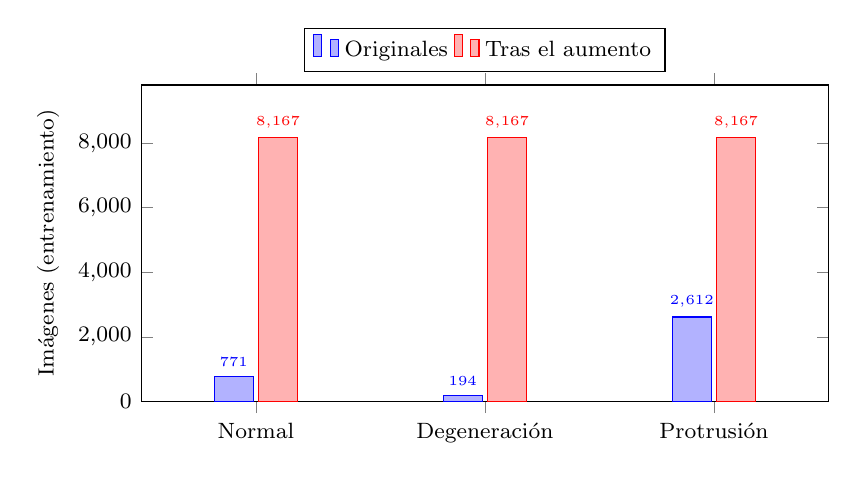
\begin{tikzpicture}
\begin{axis}[
  ybar, bar width=14pt, width=0.85\linewidth, height=5.6cm,
  symbolic x coords={Normal,Degeneración,Protrusión}, xtick=data,
  ymin=0, ymax=9800, ylabel={Imágenes (entrenamiento)},
  enlarge x limits=0.25, legend style={at={(0.5,1.04)},anchor=south,legend columns=2,font=\footnotesize},
  nodes near coords, every node near coord/.append style={font=\tiny},
  tick label style={font=\footnotesize}, ylabel style={font=\footnotesize}]
\addplot coordinates {(Normal,771) (Degeneración,194) (Protrusión,2612)};
\addplot coordinates {(Normal,8167) (Degeneración,8167) (Protrusión,8167)};
\legend{Originales, Tras el aumento}
\end{axis}
\end{tikzpicture}
\caption{Balance por conteo en entrenamiento: ROI originales y total tras el aumento.}
\label{fig:balance}
\end{figure}

\paragraph{Trazabilidad.} Cada archivo se llama \arch{T2_TSE_SAG__0188_008_L4-L5__orig.png} (original) o \arch{..._aug012.png} (copia), con paciente, corte y nivel. El manifiesto \arch{manifest_35k.csv} registra, para cada una de las 35\,007 imágenes, su partición, clase, paciente, nivel, ROI original, revisor y, en las copias, los parámetros exactos (semilla, ángulo, zoom, desplazamientos, contraste y brillo); \arch{split_pacientes.csv} guarda la partición de cada paciente. Las copias respetan los rangos declarados (ángulo entre $-8^{\circ}$ y $8^{\circ}$, zoom entre 0,90 y 1,10, contraste entre 0,90 y 1,10).

\paragraph{Verificaciones.} El script comprueba que (i) los conjuntos de pacientes de las tres particiones son disjuntos, (ii) toda copia está en la misma partición que su original, (iii) los nombres de archivo son únicos, (iv) todo PNG está íntegro y (v) el total supera los 35\,000.

\subsection{Balance de clases y sesgo por nivel}
\label{sec:balance}
El balance de 1/3 por clase es \emph{por conteo}, no por originales. Entre los 5\,123 ROI originales, la Protrusión es el 73,0\,\% (3\,738), Normal el 21,6\,\% (1\,105) y Degeneración el 5,5\,\% (280); un clasificador que siempre dijera Protrusión acertaría cerca del 73\,\%. Las copias igualan la contribución de cada clase al entrenamiento, pero no añaden anatomía nueva: el tamaño efectivo del dataset es el número de pacientes (399), y la Degeneración, repetida unas 42 veces, solo tiene 42 originales en la partición de prueba, lo que deja un margen de error amplio en su recall. Para que las métricas no se inflen con copias casi idénticas, los resultados principales se calculan sobre los \textbf{originales} de la partición de prueba, y el conjunto completo se reporta aparte. Además, un modelo entrenado con prior uniforme tiende a sobrepredecir las clases raras en la población real.

\begin{table}[t]
\centering\small
\caption{ROI originales elegibles por nivel y clase.}
\label{tab:nivel}
\begin{tabular}{lrrrrr}
\toprule
Nivel & Normal & Degeneración & Protrusión & Total & \% Protrusión \\
\midrule
L1-L2 & 505 & 121 & 401    & 1\,027 & 39,0 \\
L2-L3 & 383 & 94  & 550    & 1\,027 & 53,6 \\
L3-L4 & 172 & 44  & 811    & 1\,027 & 79,0 \\
L4-L5 & 15  & 5   & 1\,005 & 1\,025 & 98,0 \\
L5-S1 & 30  & 16  & 971    & 1\,017 & 95,5 \\
\bottomrule
\end{tabular}
\end{table}

La Tabla~\ref{tab:nivel} muestra un sesgo importante: casi toda la patología se concentra en L4-L5 y L5-S1. Un clasificador que solo adivinara la clase más frecuente de cada nivel acertaría 3\,842 de 5\,123 ROI (75,0\,\%), de modo que el nivel podría actuar como atajo. Por ello los resultados se reportan también por nivel. Esto relativiza cualquier umbral de exactitud: un 95\,\% medido sobre estas etiquetas mide acuerdo con etiquetas de estudiantes y puede alcanzarse en parte por el atajo, y cifras internas altas suelen bajar al evaluar con datos externos \cite{yi2023}. Por eso se acompaña la exactitud con F1 macro y recall por clase, que además es lo que justifica el uso de F1 con clases desbalanceadas \cite{alkubaisi2022}.

\subsection{Viabilidad del dataset}
\begin{itemize}
  \item \textbf{Disponibilidad y licencia.} Los datos son públicos y los scripts reproducen el procesamiento a partir de ellos. Las imágenes del dataset construido no se suben al repositorio: se distribuyen como un archivo comprimido de 405~MB y el repositorio guarda sus manifiestos.
  \item \textbf{Tamaño.} Cumple el requisito de más de 35\,000 registros. El contenido informativo real es menor: 5\,123 ROI de 399 pacientes, con 280 originales de Degeneración.
  \item \textbf{Balance.} Equilibrado por conteo entre las tres clases y en cada partición; desbalanceado en originales y por nivel (Secciones~\ref{sec:aumento} y~\ref{sec:balance}).
  \item \textbf{Reproducibilidad.} Semilla única (42), manifiesto por imagen y verificaciones automáticas.
  \item \textbf{Cómputo.} Los cuatro modelos se entrenaron con este mismo dataset en una GPU de consumo (RTX 3060~Ti), lo que indica que el tamaño es manejable con recursos modestos.
\end{itemize}

\subsection{Limitaciones}
(1) Las etiquetas son de estudiantes, sin radiólogo, con apoyo de un modelo, y no se midió el acuerdo entre anotadores. (2) Solo hay plano sagital; Hernia y Abombamiento no son separables y se fusionaron después de ver los datos. (3) Un único equipo de resonancia de 1,5~T, sin diversidad de escáner. (4) El tamaño efectivo son 399 pacientes; las copias no aportan anatomía nueva. (5) Degeneración cuenta con pocos pacientes (81, 17 y 22 en las tres particiones). (6) Sesgo por nivel y prior uniforme (Sección~\ref{sec:balance}). (7) Con el identificador de paciente vacío no puede descartarse la presencia de un mismo paciente en dos carpetas. (8) El conjunto es una herramienta académica, no diagnóstica.
